% This file was converted to LaTeX by Writer2LaTeX ver. 1.4
% see http://writer2latex.sourceforge.net for more info
\documentclass[a4paper]{article}
\usepackage[utf8]{inputenc}
\usepackage[T1]{fontenc}
\usepackage[ngerman]{babel}
\usepackage{amsmath}
\usepackage{amssymb,amsfonts,textcomp}
\usepackage{color}
\usepackage{array}
\usepackage{supertabular}
\usepackage{hhline}
\usepackage{hyperref}
\hypersetup{pdftex, colorlinks=true, linkcolor=blue, citecolor=blue, filecolor=blue, urlcolor=blue, pdftitle=}
\usepackage[pdftex]{graphicx}
% footnotes configuration
\makeatletter
\renewcommand\thefootnote{\arabic{footnote}}
\makeatother
% Outline numbering
\setcounter{secnumdepth}{3}
\renewcommand\thesection{\arabic{section}}
\renewcommand\thesubsection{\arabic{section}.\arabic{subsection}}
\renewcommand\thesubsubsection{\arabic{section}.\arabic{subsection}.\arabic{subsubsection}}
\makeatletter
\newcommand\arraybslash{\let\\\@arraycr}
\makeatother
% List styles
\newcommand\liststyleLSi{%
\renewcommand\labelitemi{${\bullet}$}
\renewcommand\labelitemii{${\circ}$}
\renewcommand\labelitemiii{${\blacksquare}$}
\renewcommand\labelitemiv{${\bullet}$}
}
\newcommand\liststyleLSii{%
\renewcommand\labelitemi{${\bullet}$}
\renewcommand\labelitemii{${\circ}$}
\renewcommand\labelitemiii{${\blacksquare}$}
\renewcommand\labelitemiv{${\bullet}$}
}
\newcommand\liststyleLSiii{%
\renewcommand\labelitemi{${\bullet}$}
\renewcommand\labelitemii{${\circ}$}
\renewcommand\labelitemiii{${\blacksquare}$}
\renewcommand\labelitemiv{${\bullet}$}
}
\newcommand\liststyleLSiv{%
\renewcommand\labelitemi{${\bullet}$}
\renewcommand\labelitemii{${\circ}$}
\renewcommand\labelitemiii{${\blacksquare}$}
\renewcommand\labelitemiv{${\bullet}$}
}
\newcommand\liststyleLSv{%
\renewcommand\labelitemi{${\bullet}$}
\renewcommand\labelitemii{${\circ}$}
\renewcommand\labelitemiii{${\blacksquare}$}
\renewcommand\labelitemiv{${\bullet}$}
}
\newcommand\liststyleLSvi{%
\renewcommand\labelitemi{${\bullet}$}
\renewcommand\labelitemii{${\circ}$}
\renewcommand\labelitemiii{${\blacksquare}$}
\renewcommand\labelitemiv{${\bullet}$}
}
\newcommand\liststyleLSvii{%
\renewcommand\labelitemi{${\bullet}$}
\renewcommand\labelitemii{${\circ}$}
\renewcommand\labelitemiii{${\blacksquare}$}
\renewcommand\labelitemiv{${\bullet}$}
}
\newcommand\liststyleLSviii{%
\renewcommand\labelitemi{${\bullet}$}
\renewcommand\labelitemii{${\circ}$}
\renewcommand\labelitemiii{${\blacksquare}$}
\renewcommand\labelitemiv{${\bullet}$}
}
\newcommand\liststyleLSix{%
\renewcommand\labelitemi{${\bullet}$}
\renewcommand\labelitemii{${\circ}$}
\renewcommand\labelitemiii{${\blacksquare}$}
\renewcommand\labelitemiv{${\bullet}$}
}
\newcommand\liststyleLSx{%
\renewcommand\labelitemi{${\bullet}$}
\renewcommand\labelitemii{${\circ}$}
\renewcommand\labelitemiii{${\blacksquare}$}
\renewcommand\labelitemiv{${\bullet}$}
}
\newcommand\liststyleLSxi{%
\renewcommand\labelitemi{${\bullet}$}
\renewcommand\labelitemii{${\circ}$}
\renewcommand\labelitemiii{${\blacksquare}$}
\renewcommand\labelitemiv{${\bullet}$}
}
\newcommand\liststyleLSxii{%
\renewcommand\labelitemi{${\bullet}$}
\renewcommand\labelitemii{${\circ}$}
\renewcommand\labelitemiii{${\blacksquare}$}
\renewcommand\labelitemiv{${\bullet}$}
}
\newcommand\liststyleLSxiii{%
\renewcommand\labelitemi{${\bullet}$}
\renewcommand\labelitemii{${\circ}$}
\renewcommand\labelitemiii{${\blacksquare}$}
\renewcommand\labelitemiv{${\bullet}$}
}
\newcommand\liststyleLSxiv{%
\renewcommand\labelitemi{${\bullet}$}
\renewcommand\labelitemii{${\circ}$}
\renewcommand\labelitemiii{${\blacksquare}$}
\renewcommand\labelitemiv{${\bullet}$}
}
\newcommand\liststyleLSxv{%
\renewcommand\labelitemi{${\bullet}$}
\renewcommand\labelitemii{${\circ}$}
\renewcommand\labelitemiii{${\blacksquare}$}
\renewcommand\labelitemiv{${\bullet}$}
}
\newcommand\liststyleLSxvi{%
\renewcommand\theenumi{\arabic{enumi}}
\renewcommand\theenumii{\alph{enumii}}
\renewcommand\theenumiii{\roman{enumiii}}
\renewcommand\theenumiv{\arabic{enumiv}}
\renewcommand\labelenumi{\theenumi.}
\renewcommand\labelenumii{\theenumii.}
\renewcommand\labelenumiii{\theenumiii.}
\renewcommand\labelenumiv{\theenumiv.}
}
\newcommand\liststyleLSxvii{%
\renewcommand\labelitemi{${\bullet}$}
\renewcommand\labelitemii{${\circ}$}
\renewcommand\labelitemiii{${\blacksquare}$}
\renewcommand\labelitemiv{${\bullet}$}
}
\newcommand\liststyleLSxviii{%
\renewcommand\labelitemi{${\bullet}$}
\renewcommand\labelitemii{${\circ}$}
\renewcommand\labelitemiii{${\blacksquare}$}
\renewcommand\labelitemiv{${\bullet}$}
}
% Page layout (geometry)
\setlength\voffset{-1in}
\setlength\hoffset{-1in}
\setlength\topmargin{2cm}
\setlength\oddsidemargin{3.5cm}
\setlength\textheight{22.706001cm}
\setlength\textwidth{15.500999cm}
\setlength\footskip{1.497cm}
\setlength\headheight{0.998cm}
\setlength\headsep{0.499cm}
% Footnote rule
\setlength{\skip\footins}{0.119cm}
\renewcommand\footnoterule{\vspace*{-0.018cm}\setlength\leftskip{0pt}\setlength\rightskip{0pt plus 1fil}\noindent\textcolor{black}{\rule{0.25\columnwidth}{0.018cm}}\vspace*{0.101cm}}
% Pages styles
\makeatletter
\newcommand\ps@Standard{
  \renewcommand\@oddhead{\sffamily INM - Potentielle Neuordnung des Informationsmanagements\hfill 25.05.15}
  \renewcommand\@evenhead{\@oddhead}
  \renewcommand\@oddfoot{\sffamily INM – SoSe 2015\hfill \hfill \thepage{} / ?}
  \renewcommand\@evenfoot{\@oddfoot}
  \renewcommand\thepage{\arabic{page}}
}
\makeatother
\pagestyle{Standard}
\setlength\tabcolsep{1mm}
\renewcommand\arraystretch{1.3}
% Non-floating captions
\makeatletter
\newcommand\captionof[1]{\def\@captype{#1}\caption}
\makeatother
\title{}
\begin{document}
\setcounter{tocdepth}{4}
\renewcommand\contentsname{Inhaltsverzeichnis}
\tableofcontents
\section*{}
\clearpage\section{Kostenarten}
\label{bkm:RefHeading24765162299686}
\bigskip

{\sffamily
Kalkulationen benötigt bestimmte eindeutige Kostenarten, die dann in einem Kostenartenplan aufgestellt und in einer
Kostenartenrechnung kontrolliert werden können. Die eindeutige Kostenarten können in Kostenartenkategorien bzw.
Kostenartengruppen zusammen fließen. \ Im folgenden soll einmal festgehalten werden, was man für die Kalkulation nutzen
sollte.}

{\centering 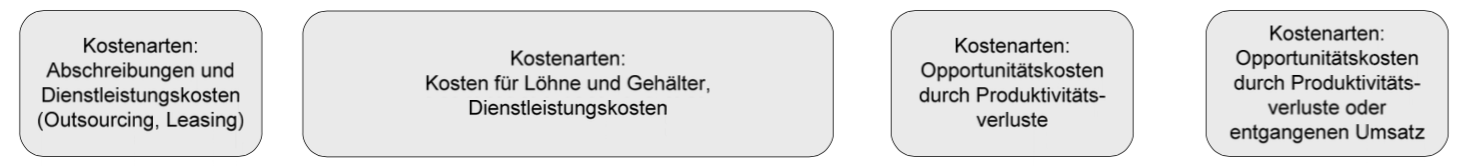
\includegraphics[width=15.455cm,height=1.75cm]{INMAusarbeitung02-img001.png}
\captionof{figure}[Beispiel von Kostenarten in der TCO{}-Methode (Hansen 2009)]{Beispiel von Kostenarten in der
TCO-Methode \textcolor{red}{(Hansen 2009)}}
\label{seq:refIllustration0}
\par}
{\sffamily
Die Kostenarten der \figurename~\ref{seq:refIllustration0} finden sich z.B. in der von Krcmar benannten TCO-Methode
(“Total Cost of Ownership”) wieder. Aus den bewerteten Daten der Kostenarten können periodische Durchschnittswerte
ermittelt werden, aus denen dann für die Zukunft neue Abschätzungen gewonnen werden.}

{\sffamily
In einer ABC-Analyse kann eine weitere Klassifizierung vorgenommen werden, um z.B. aufzuzeigen welche Kostenarten auf
jeden Fall (A-Klasse) anfallen, welche im besten Fall noch erledigt werden sollen (B-Klasse) und welche man optional
(C-Klasse) aufwenden sollte.}


\bigskip

{\sffamily
Die Kostenarten der \tablename~\ref{seq:refTable0} sind die Grundelemente der Wertsteigerung durch Wertschöpfung, die in
die Kostenartenrechnung fließen sollten. „Die Kostenartenrechnung erfasst, systematisiert und periodisiert die
Kosten.“\footnote{[REI15]} Die Kostenarten der \tablename~\ref{seq:refTable0} sollen in diesem Projekt als Übersicht
dienen, da aktuell nur drei Module in der Kostenschätzung betrachtet werden, für den Fall das weitere Module
abzuschätzen sind.}


\bigskip


\bigskip

\begin{center}
\bottomcaption[Gliederungsmo\"{ }glichkeiten der Kostenarten ( Reim 2015)]{Gliederungsm\"{o}glichkeiten der Kostenarten
\textcolor[rgb]{1.0,0.2,0.2}{( }\textcolor{red}{Reim 2015)}}
\label{seq:refTable0}\tablefirsthead{}
\tablehead{}
\tabletail{}
\tablelasttail{}
\begin{supertabular}{|m{7.5360003cm}|m{7.563cm}|}
\hline
{\sffamily\bfseries\color{black} Gliederungsmerkmale nach} &
{\sffamily\bfseries\color{black} Kostenartengruppen}\\\hline
{\sffamily\color{black} der Zahlungswirksamkeit} &
\liststyleLSi
\begin{itemize}
\item {\sffamily\color{black} Grundkosten}
\item {\sffamily\color{black} kalkulatorischen Kosten}
\end{itemize}
\\\hline
{\sffamily\color{black} der Art der verbrauchten Einsatzgüter}

~
 &
\liststyleLSii
\begin{itemize}
\item {\sffamily\color{black} Materialkosten}
\item {\sffamily\color{black} Personalkosten}
\item {\sffamily\color{black} Fremdleistungskosten}
\item {\sffamily\color{black} (Kalkulatorische) Abschreibungen}
\item {\sffamily\color{black} (Kalkulatorische) Kapitalkosten}
\item {\sffamily\color{black} Kalkulatorische Zusatzkosten}
\item {\sffamily\color{black} Kostensteuern und Gebühren}
\end{itemize}
\\\hline
{\sffamily\color{black} der Herkunft der verbrauchten\newline
Einsatzgüter} &
\liststyleLSiii
\begin{itemize}
\item {\sffamily\color{black} Primäre Kosten}
\item {\sffamily\color{black} Sekundäre Kosten}
\end{itemize}
\\\hline
{\sffamily\color{black} den Funktionsbereichen} &
\liststyleLSiv
\begin{itemize}
\item {\sffamily\color{black} Beschaffungskosten}
\item {\sffamily\color{black} Fertigungskosten}
\item {\sffamily\color{black} Vertriebskosten}
\item {\sffamily\color{black} Forschungs- u. Entwicklungskosten}
\item {\sffamily\color{black} Verwaltungskosten}
\end{itemize}
\\\hline
{\sffamily\color{black} der Beschäftigungsabhängigkeit} &
\liststyleLSv
\begin{itemize}
\item {\sffamily\color{black} Variable Kosten}
\item {\sffamily\color{black} Fixe Kosten}
\end{itemize}
\\\hline
{\sffamily\color{black} der Art der Verrechnung} &
\liststyleLSvi
\begin{itemize}
\item {\sffamily\color{black} Einzelkosten}
\item {\sffamily\color{black} Gemeinkosten}
\item {\sffamily\color{black} Sondereinzelkosten}
\end{itemize}
\\\hline
\end{supertabular}
\end{center}
\subsection[\ Kostenarten in Hochschulen]{\ Kostenarten in Hochschulen}
{\sffamily
Im Hochschulbereich betrachtet man besonders die Kostenarten der Einzelkosten und Gemeinkosten. Die Kostenarten müssen,
im universitären Umfeld, besonders in Forschungsprojekten mit Drittmitteln genau aufgeschlüsselt und zugewiesen werden,
um einen transparenten Überblick zu erhalten, wo die Kosten anfallen und wo die Drittmittel
hinfließen\footnote{[PKL05]}.}


\bigskip

{\sffamily
Die genaue Form der Kostenerfassung sollte in diesem Projekt angewendet werden. Es sollte eine sekundäre Kostenart
Informationsmanagement geben, damit die Kosten zugeordnet und überwacht werden können. Daraus können folgende Projekte
im Vorfeld besser eingeschätzt werden. Dies wird durch die Einzelkosten erreicht, wohingegen die Gemeinkosten in
mehreren Bereichen der Hochschule anfallen und der Aufwand einer Einzelzuordnung nicht vertretbar oder zielführend
ist.}


\bigskip

{\sffamily
Die kalkulatorischen Kosten teilen sich in die Zusatzkosten und die Anderskosten und sind in der
\figurename~\ref{seq:refIllustration1} tabellarisch eingeordnet. Anderskosten sind Kostenarten die noch nicht benannt
sind bzw. erkannt werden, aber nicht in der laufenden Periode zugeordnet werden können. }

{\centering 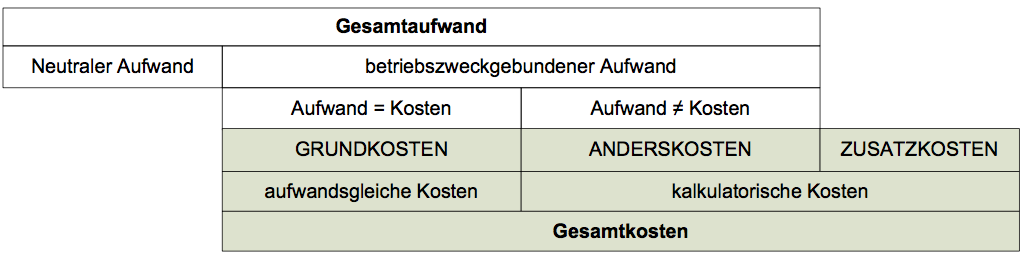
\includegraphics[width=15.455cm,height=3.963cm]{INMAusarbeitung02-img002.png}
\captionof{figure}[Abgrenzung Aufwand {}- Kosten (Handbuch Kostenartenrechnung 05)]{Abgrenzung Aufwand -
Kosten\textcolor[rgb]{1.0,0.2,0.2}{ (Handbuch Kostenartenrechnung 05}\textcolor{red}{)}}
\label{seq:refIllustration1}
\par}
{\sffamily
In der Betrachtung der primären und sekundären Kostenarten, sind in einer Hochschule die sekundären Kostenarten
besonders interessant, da sie die Kosten der Bereiche zusammenfassen und einen Überblick verschaffen.\newline
Wie das Beispiel der \figurename~\ref{seq:refIllustration2} zeigt, bauen sich die sekundären Kosten, in der
Kostenstellenrechung, durch das Zusammenfließen der primären Kosten auf. An der Leibnitz Universität Hannover (LUH)
wurden, für das SAP-System, 900 Primärkostenarten in 140 Sekundärkostenarten verdichtet und
zugeordnet\footnote{[PKL05]}.}

{\centering 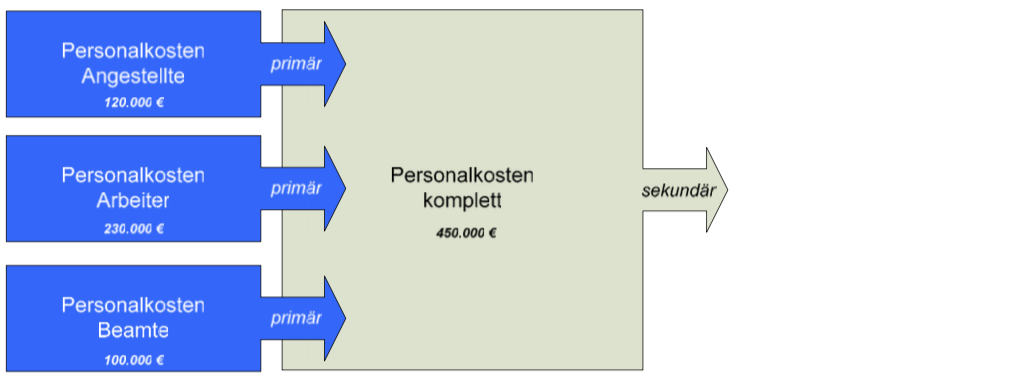
\includegraphics[width=11.67cm,height=5.884cm]{INMAusarbeitung02-img003.png}
\captionof{figure}[U\"{ }bergang von Prima\"{ }r{}- in Sekunda\"{ }rkostenarten (Handbuch Kostenartenrechnung
05)]{\"{U}bergang von Prim\"{a}r- in Sekund\"{a}rkostenarten\textcolor[rgb]{1.0,0.2,0.2}{ (Handbuch Kostenartenrechnung
05}\textcolor{red}{)}}
\label{seq:refIllustration2}
\par}
{\sffamily
Diese Primärkostenarten und Sekundärkostenarten sind im Jahr 2005 im Rahmen des Projektes “Uni2001” für ganz
Niedersachsen abgestimmt worden und im SAP-System eingepflegt. Ein entsprechender Abgleich mit Mitarbeitern der
Hochschule Emden/Leer für die vorhandenen und besonders der genutzten Kostenarten sollte bei der konkreten
Projektplanung unbedingt erfolgen. Die Hierarchie der Kostenarten der Hochschule sollten sich ähnlich, wenn nicht sogar
gleich, dem Beispiel der \figurename~\ref{seq:refIllustration3} der LUH darstellen.}

{\centering 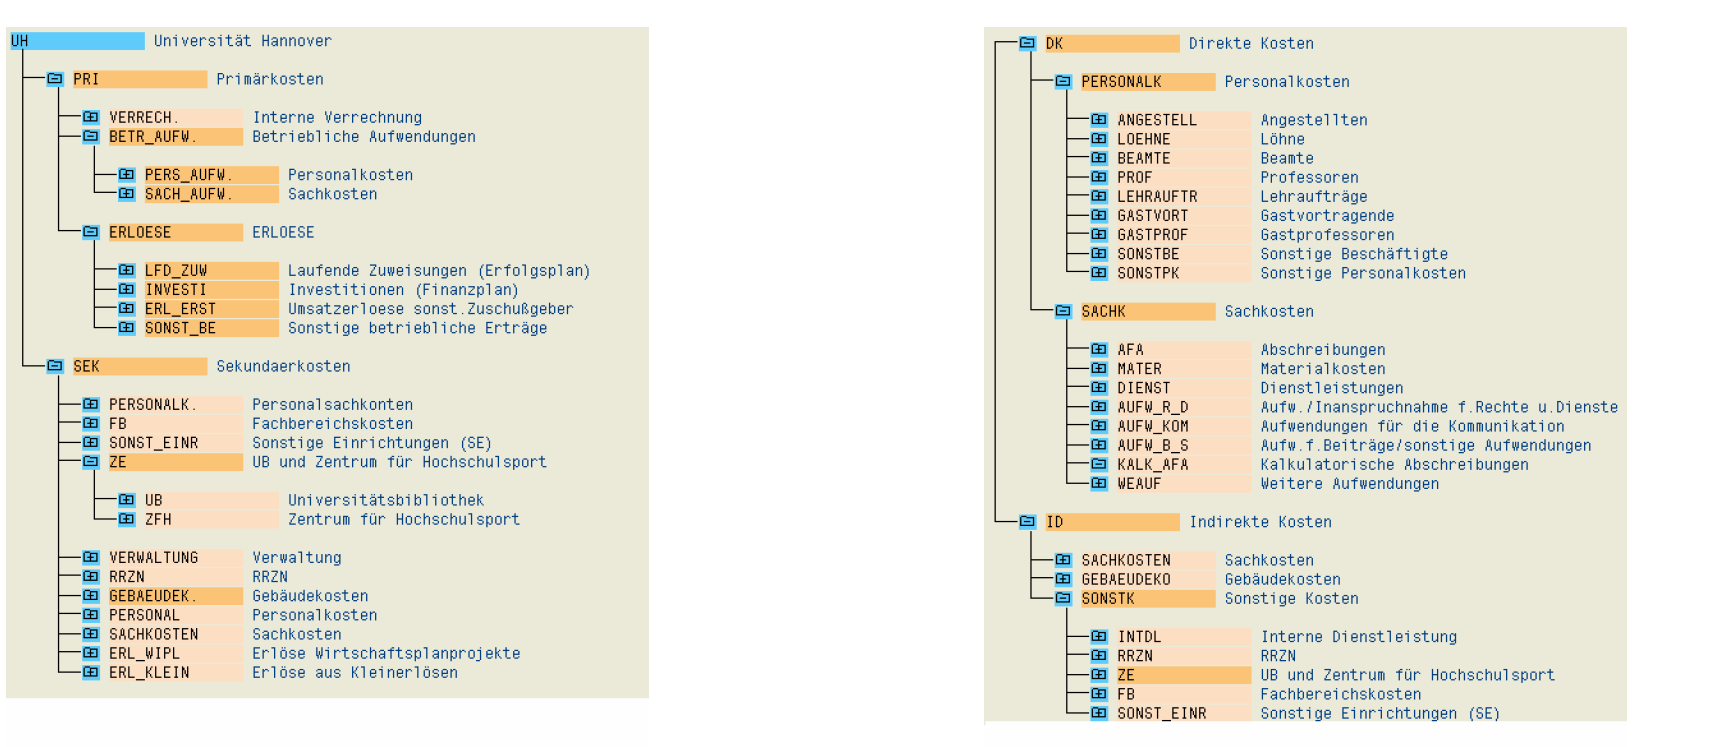
\includegraphics[width=15.385cm,height=6.706cm]{INMAusarbeitung02-img004.png}
\captionof{figure}[ \ Kostenartenhierarchie der Hochschulen Uni2001 (Handbuch Kostenartenrechnung 05)]{
\ Kostenartenhierarchie der Hochschulen Uni2001\textcolor[rgb]{1.0,0.2,0.2}{ (Handbuch Kostenartenrechnung
05}\textcolor{red}{)}}
\label{seq:refIllustration3}
\par}
\subsection*{}
\clearpage\subsection{Kostenarten in der IT}
{\sffamily
In einer Hochschule ist ein Rechenzentrum für die Aufgaben der IT zuständig.\newline
Der Rechenzentrumsleiter ist in einem Netzwerk, aus leitenden Personen der Hochschule, das Zentrum der personellen
IT-Komponenten. Im Bereich der IT einer Hochschule wird im Bereich der direkten Kosten zwischen den
Prim\"{a}rkategorien Hard- und Software, operativer Betrieb und Verwaltung differenziert\footnote{[HAN09]}.}


\bigskip

{\sffamily
Zusätzlich ist ein Rechenzentrum der Hochschule, nach Interview-Aussage des Rechenzentrumsleiters der Hochschule
Emden/Leer, jährlich auf ein bestimmtes Budget festgelegt. Dabei ist die \tablename~\ref{seq:refTable1} zu beachten
welche Kosten budgetiert werden können und welche nicht.}


\bigskip

\begin{table}
\centering
\begin{tabular}{|m{7.2980003cm}|m{7.8010006cm}|}

\hline
{\sffamily\bfseries\color{black} Budgetierte Kosten} &
{\sffamily\bfseries\color{black} Nicht budgetierte Kosten}\\\hline
{\sffamily\color{black} Software-Entwicklung}

\liststyleLSvii
\begin{itemize}
\item {\sffamily\color{black} Neuentwicklung und \newline
Anpassungen}
\item {\sffamily\color{black} Personal- und Sachkosten}
\end{itemize}
 &
{\sffamily\color{black} Negative Produktivitätseffekte}

\liststyleLSviii
\begin{itemize}
\item {\sffamily\color{black} Antwort-, Rüst- und Bearbeitungszeit}
\item {\sffamily\color{black} Motivation}
\item {\sffamily\color{black} Ergonomie}
\end{itemize}
\\\hline
{\sffamily\color{black} Kommunikation}

\liststyleLSix
\begin{itemize}
\item {\sffamily\color{black} Netzwerk}
\item {\sffamily\color{black} Personal- und Sachkosten}
\end{itemize}
 &
{\sffamily\color{black} Ausfall}

\liststyleLSx
\begin{itemize}
\item {\sffamily\color{black} geplant}
\item {\sffamily\color{black} ungeplant}
\end{itemize}
\\\hline
{\sffamily\color{black} Hardware/Software}

\liststyleLSxi
\begin{itemize}
\item {\sffamily\color{black} Abschreibung, Miete und Leasing}
\item {\sffamily\color{black} Entsorgung}
\item {\sffamily\color{black} Client/Server}
\item {\sffamily\color{black} Administration}
\end{itemize}
 &
{\sffamily\color{black} Endbenutzer}

\liststyleLSxii
\begin{itemize}
\item {\sffamily\color{black} Peer-Support (selbst/gegenseitig)}
\item {\sffamily\color{black} Unproduktives Konfigurieren}
\item {\sffamily\color{black} Qualifizierung (selbst/gegenseitig)}
\end{itemize}
\\\hline
{\sffamily\color{black} Support}

\liststyleLSxiii
\begin{itemize}
\item {\sffamily\color{black} Help-Desk}
\item {\sffamily\color{black} Personal-, Sach- und \newline
Gemeinkosten}
\item {\sffamily\color{black} Intern/Extern}
\item {\sffamily\color{black} Schulung Intern/Extern}
\end{itemize}
 &
~
\\\hline
{\sffamily\color{black} Systembetrieb und Systemmanagement}

\liststyleLSxiv
\begin{itemize}
\item {\sffamily\color{black} Verwaltung}
\item {\sffamily\color{black} Installation/Optimierung}
\item {\sffamily\color{black} Instandhaltung}
\end{itemize}
 &
~
\\\hline\end{tabular}
\caption[Auswahl IT{}-Kostenarten nach Krcmar ( Krcmar 2015)]{Auswahl IT-Kostenarten nach
Krcmar\textcolor[rgb]{1.0,0.2,0.2}{ ( }\textcolor{red}{Krcmar 2015)}}
\label{seq:refTable1}
\end{table}

\bigskip


\bigskip

\clearpage{\sffamily
Als spezielle IT-Kostenarten werden von Gadatsch und Mayer\footnote{[GAD14]}\textcolor{red}{ }aufgelistet:}


\bigskip

\begin{table}
\centering
\begin{tabular}{|m{7.545cm}|m{6.228cm}|}

\hline
{\sffamily\bfseries\color{black} Sekundäre Kostenarten} &
{\sffamily\bfseries\color{black} Primäre Kostenarten}\\\hline
{\sffamily\color{black} Hardware-Kosten} &
\liststyleLSxv
\begin{itemize}
\item {\sffamily\color{black} Miete/Leasing}
\item {\sffamily\color{black} Hardware}
\item {\sffamily\color{black} Leitungsgebühren}
\item {\sffamily\color{black} Wartung}
\end{itemize}
\\\hline
{\sffamily\color{black} Software-Kosten} &
\liststyleLSxv
\begin{itemize}
\item {\sffamily\color{black} Miete/Leasing}
\item {\sffamily\color{black} Software}
\item {\sffamily\color{black} eigene Entwicklung}
\item {\sffamily\color{black} Externe Wartung}
\item {\sffamily\color{black} Beratung}
\end{itemize}
\\\hline
{\sffamily\color{black} Daten-Kosten} &
\liststyleLSxv
\begin{itemize}
\item {\sffamily\color{black} Beratung}
\item {\sffamily\color{black} Kauf}
\end{itemize}
\\\hline
{\sffamily\color{black} Sonstige IT-Kosten} &
\liststyleLSxv
\begin{itemize}
\item {\sffamily\color{black} IT-Verbrauchsmaterial}
\item {\sffamily\color{black} IT-Versicherungen}
\item {\sffamily\color{black} Beiträge zu Fachverbänden}
\item {\sffamily\color{black} IT-Fachliteratur}
\item {\sffamily\color{black} IT-Schulungen}
\end{itemize}
\\\hline
{\sffamily\color{black} Innerbetriebliche IT-Leistungsverrechnung } &
\liststyleLSxv
\begin{itemize}
\item {\sffamily\color{black} Umlagen}
\item {\sffamily\color{black} Entwicklungskosten}
\item {\sffamily\color{black} Benutzerservice}
\end{itemize}
\\\hline\end{tabular}
\caption[Auflistung der speziellen IT{}-Kosten \ ( Gadatsch \& Mayer 2015)]{Auflistung der speziellen IT-Kosten
\textcolor[rgb]{1.0,0.2,0.2}{\ ( }\textcolor{red}{Gadatsch \& Mayer 2015)}}
\label{seq:refTable2}
\end{table}

\bigskip

{\sffamily
Die Kostenarten aus den Auflistungen der \tablename~\ref{seq:refTable1} und \tablename~\ref{seq:refTable2}eignen sich
für die Betrachtung der Kosten an einer Hochschule\footnote{[HAN09]}. }


\bigskip


\bigskip

\clearpage{\sffamily
Im Bezug auf die Kostenarten schlägt Krcmar z.B. die TCO-Methode (“Total Cost of Ownership”) als Bewertungstechnik vor,
was auch im nächsten Kapitel beschrieben und verwendet wird\footnote{[KRC15]}. Die TCO-Methode nutzt die Kostenarten,
um die wirtschaftlichen Auswirkungen in der IT aufzuzeigen.}


\bigskip

{\sffamily
Vor allem im Bezug auf Kostenarten und IT wird als Trend ein IT-Controller empfohlen, um eine bessere Wertschöpfung in
der IT zu erreichen, was im Blick auf die Kostenart Personal einen wirtschaftlichen Vorteil bewirkt. Der IT-Controller
sollte jedoch nicht in einer rein bestimmenden Funktion auftreten, sondern eher als Motivator für mehr Effizienz,
Ergonomie und Effektivität, was im Umkehrschluss bessere Arbeitsbedingungen und damit auch mehr Erfolg für Projekte
bringt\footnote{[REI15]}.}


\bigskip

{\sffamily
Gerade in einem solch zentralen Projekt mit einem hohen Anteil an IT-lastigen Themen ist es zumindest empfehlenswert
über einen IT-Controller nachzudenken\footnote{[STR13]}. Besonders ist hier auch die höhere Komplexität zu beachten,
die im Verlauf der Zeit in der IT der DFG-Referenzprojekte entstanden. Die Projekte werden im Kapitel
\ref{bkm:RefHeading24761162299686} vorgestellt bzw. genannt.}

\clearpage\section{Verfahren für Kosten- und Zeitschätzung}
{\sffamily
Nachdem in Kapitel \ref{bkm:RefHeading24765162299686} die für diese Arbeit relevanten Kostenarten beleuchtet wurden,
werden in diesem Kapitel Möglichkeiten aufgezeigt, um die Kosten und die zur Realisierung benötigte Zeit zu schätzen.
Im weiteren Verlauf werden Planungs- und Überwachungsinstrumente des Projektmanagements erläutert, die für das
durchzuführende Projekt am geeignetsten scheinen. Dabei liegt der Fokus vor allem auf einer möglichst agilen Umsetzung
des Projekts. Abschließend werden die untersuchten Verfahren beispielhaft auf drei konkrete Komponenten des Projekts
angewendet.}

\subsection{Projektmanagement an einer Hochschule}
\label{bkm:RefNumPara23461511499216}{\sffamily
Wie bereits in \textcolor[rgb]{1.0,0.2,0.2}{Kapitel X.X (Besonderheiten an Hochschulen)}\textcolor{blue}{
}\ beschrieben, weißt eine Hochschule als Organisation eine Reihe von Besonderheiten auf. Für das Projektmanagement
bedeutet besonders die Tatsache, dass die einzelnen Fachbereiche ein hohes Maß an Autonomie und
Entscheidungskompetenzen besitzen, eine entsprechend angepasst Herangehensweise\footnote{[HAN09]}.}


\bigskip

{\sffamily
Die zentrale Herausforderung des Projektmanagements ist es, die Interessen der unterschiedlichen Verwaltungsbereiche,
der späteren Nutzer und der Hochschulleitung zu wahren und zu vereinen. Durch die Autonomie der Fachbereiche und deren
unterschiedlichen Interessen ist es möglich, dass sich innerhalb der Hochschule konkurrierende Arbeitsgruppen bilden.
Es ist daher eine weitere, nicht zu unterschätzende, Aufgabe des Projektmanagements, die Kommunikation zwischen allen
beteiligten Arbeitsgruppen, möglichen externen Akteuren und dem akademischen Bereich aufrecht zu erhalten und zu
fördern\footnote{[ALT07]}.}


\bigskip

{\sffamily
Des Weiteren führen umfangreiche Änderungen in Organisationen oftmals zu einer besonderen Eigendynamik, welche, im
Zusammenspiel mit den aufgeführten Besonderheiten einer Hochschule, zu nicht kalkulierbaren oder unvorhersehbaren
Geschehnisse führen kann. Der Umstand, dass zu Projektbeginn in der Regel noch nicht alle, für eine exakte Planung
benötigten, Informationen zur Verfügung stehen, erschwert zusätzlich die zufriedenstellende Organisation des
Projektverlaufs. Um dem entgegen zu wirken ist es empfehlenswert, dass Projekt in iterativ-reflexiven Schleifen mit
ausreichender Flexibilität durchzuführen\footnote{[HAN09]}.}


\bigskip

{\sffamily
Durch diese gewonnene Flexibilität sind Anpassungen während der Ausführung des Projektes möglich und auf besondere
Befindlichkeiten kann eingegangen werden. Durch eine iterative Durchführung wird außerdem dem Vorhaben Rechnung
getragen, dass nach jeder Umsetzung einer Komponente über den weiteren Verlauf des Projekts reflektiert werden kann.}

\subsection{Kostenschätzung (Total Cost of Ownership)}
\label{bkm:RefHeading24769162299686}{\sffamily
Neben der Organisation und Durchführung des Projekts bildet die Schätzung der Kosten im Vorfeld eine weitere wichtige
Säule des Projektmanagements. Eine möglichst ganzheitliche und realistische Erfassung aller potentiell entstehenden
Kosten ist dabei notwendig, um die Entscheidung für oder gegen ein Projekt anhand fundierter Informationen treffen zu
können.}


\bigskip

{\sffamily
Das Total-Cost-Of-Ownership-Konzept wurde im Rahmen einer Studie der Gartner Group zur vollständigen Erfassung der
direkten und indirekten Kosten\textbf{ }eines PC-Arbeitsplatzes entwickelt. Das Ergebnis der Studie hat dabei gezeigt,
dass nur ca. 20\% der Gesamtkosten tatsächlich auf die direkten Anschaffungskosten von Hard- und Software entfallen.
Der Großteil der entstehenden Kosten wird folglich durch den Einführungsprozess neuer Systeme und den langfristigen
Betrieb selbiger verursacht. Der Einsatz der TCO-Methode kann demnach dabei helfen, ein Bewertungsobjekt mit allen
zugehörigen, kostenverursachenden Aspekten zu erfassen und zu bewerten\footnote{[HAN09]}.}


\bigskip

{\sffamily
Die Tatsache, dass es sich bei dem untersuchten Studienobjekt lediglich um einen “wenig komplexen” PC-Arbeitsplatz
handelt, lässt vermuten, dass bei Einführung komplexer Systeme (z.B. Dokumentenmanagement) der Anteil der
Anschaffungskosten über den gesamten Lebenszyklus des Systems weiter schrumpft, während beispielsweise Inbetriebnahme,
Wartung und Schulung wesentlich mehr Kosten verursachen. Dieser Zusammenhang verdeutlicht die Wichtigkeit der
ganzheitlichen Kostenbetrachtung und rechtfertigt den Einsatz des TCO-Konzepts, welches es zum Ziel hat, den
Vollständigkeitsgrundsatz der Kostenrechnung\footnote{[GRO04]}\textcolor{red}{ }zu erfüllen.}


\bigskip

{\sffamily
Grundsätzlich wird im Rahmen der TCO-Aanalyse zwischen direkten und indirekten, bzw. budgetierten und
nicht-budgetierten, Kosten unterschieden. In die Kategorie der direkten Kosten fallen dabei alle Investitionen, die zur
Beschaffung und Bereitstellung der IT-Komponente notwendig sind. Die Bezeichnung als budgetierte Kosten liegt darin
begründet, dass selbige einem konkreten Bereich (z.B. Hochschulrechenzentrum bei Anschaffung eines neuen Servers)
zugeschrieben werden können. Im Gegensatz dazu handelt es sich bei indirekten Kosten um Ausgaben, die außerhalb des
Bereichs auftreten, der die direkten Kosten zu tragen hat, wodurch sie keinem konkreten Budget zugeschrieben werden
können. Eine generische Übersicht der direkten und indirekten Kategorien zeigt
\figurename~\ref{seq:refIllustration4}\footnote{[HAN09]}.}


\bigskip

{\centering 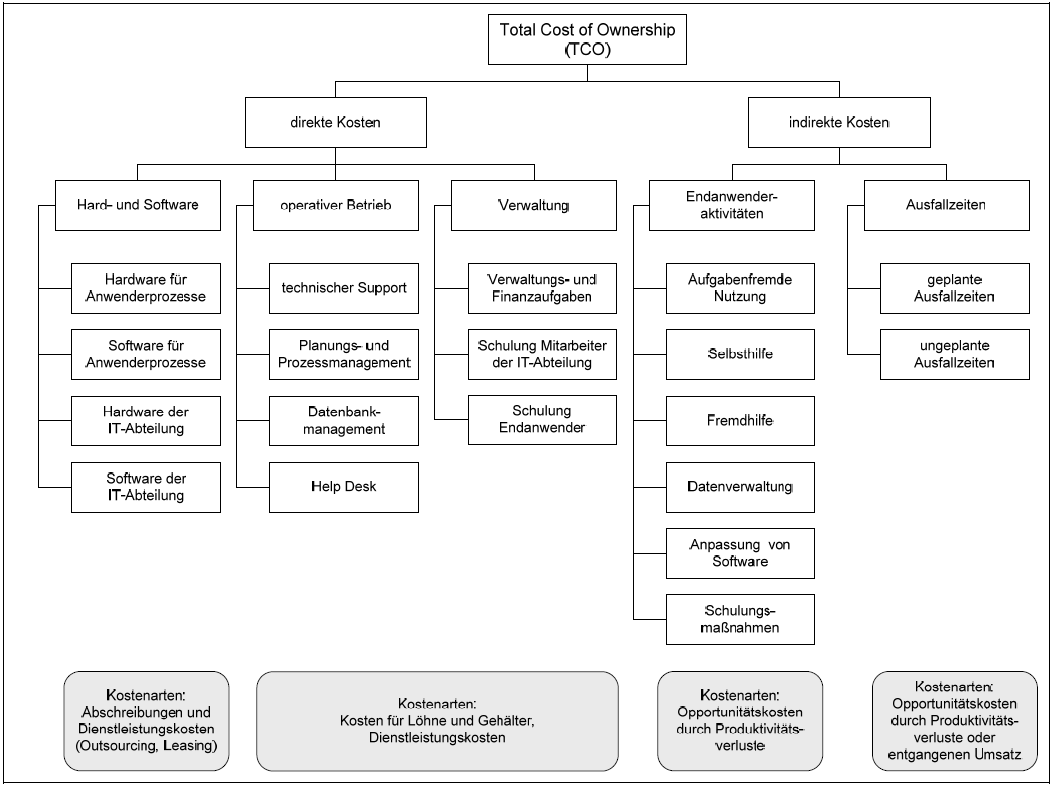
\includegraphics[width=15.45cm,height=11.555cm]{INMAusarbeitung02-img005.png}
\captionof{figure}[: \ generische Kostenkategorien {}-und Arten (Hanser 09)]{: \ generische Kostenkategorien -und Arten
\textcolor[rgb]{1.0,0.2,0.2}{(Hanser 09)}}
\label{seq:refIllustration4}
\par}
{\sffamily
Während die im Diagramm dargestellten direkten Kosten auch direkt in der IT-Abteilung anfallen und nachvollziehbar,
beziehungsweise durch angemessenen Aufwand berechenbar, sind, entstehen die indirekten Kosten in der Regel durch
Endanwender und deren “unsachgemäße Nutzung” der bereitgestellten Infrastruktur. Dies ist theoretisch bereits dann der
Fall, wenn ein Mitarbeiter einen anderen Mitarbeiter bei der Lösung von IT-Problemen unterstützt, obwohl dies nicht
seine eigentliche Aufgabe ist. Durch diese Arbeiten außerhalb seines Zuständigkeitsbereichs werden die eigentlichen
Kernaktivitäten des Mitarbeiters vernachlässigt, wodurch seine Produktivität sinkt. Dieser Produktivitätsverlust wird
durch sogenannte Opportunitätskosten abgebildet und als indirekten Kosten erfasst.}


\bigskip

{\sffamily
Die Erhebung der Informationen, die notwendig sind, um indirekte Kosten beziffern zu können, kann sich jedoch als
äußerst schwierig und zeitaufwendig herausstellen. Aufgrund fehlender formalisierter Techniken zur Erfassung eben
dieser Positionen, empfiehlt die Gartner Group den Einsatz von Befragungen und Fokusgruppen, was neben dem bereits
erwähnten, hohen zeitlichen Aufwand, außerdem zu Problemen hinsichtlich der Validität der Daten führen
kann\footnote{[HAN09]}.}


\bigskip

{\sffamily
Ferner besteht die Gefahr, dass durch die Berücksichtigung von Opportunitätskosten der in Kapitel
\ref{bkm:RefNumPara23461511499216} beschriebene, notwendige Austausch und Kontakt zwischen verschiedenen Arbeitsgruppen
und Fachbereichen stark eingeschränkt wird. Deshalb sollte in diesem speziellen, nicht-industriellen, Fall einer
Hochschule auf die initiale Berücksichtigung der indirekten Kosten verzichtet werden. Im späteren Projektverlauf,
nachdem das Zusammenspiel aller Akteure etabliert und gefestigt ist, muss jedoch versucht werden, diese Daten zu
evaluieren und in die Kalkulation mit einzubeziehen.}


\bigskip

{\sffamily
Eine beispielhafte Kalkulation auf Grundlage der TCO-Methode der Gartner Group wird in Kapitel
\ref{bkm:RefHeading24767162299686} durchgeführt. Als unterstützende Software zur Berechnung dient die kostenlose
Anwendung TCO-Tool\footnote{Download unter http://sourceforge.net/projects/tcotool/}.}

\subsection{Zeitplanung}
{\sffamily
Neben der Einschätzung der zu erwarteten Kosten soll der zeitliche Ablauf der einzelnen Projektkomponenten beleuchtet
werden. Die aufsummierte Dauer der einzelnen Komponenten ergibt dann den gesamten zeitlichen Aufwand Projekts. Zur
zeitlichen Planung der erforderlichen Schritte, sowie der Ablaufplanung einzelner Arbeitspakete werden Gantt-Diagramme
eingesetzt. Die Anwendung eines solchen Gantt-Diagramms stellt das erste Kapitel dieses Abschnitts dar. Die Einhaltung
der zuvor definierten Meilensteine und Arbeitsschritte wird dabei anhand der Meilensteintrendanalyse durchgeführt. Wie
die Meilensteintrendanalyse zur Überwachung der Projektmodule eingesetzt werden soll wird im zweiten Teil dieses
Kapitels erklärt. }

\subsubsection[Gantt{}-Diagramm]{\color{black} Gantt-Diagramm}
{\sffamily
Zur Erstellung eines Gantt-Diagramms ist es wichtig, zunächst eine Aktivitätenliste zu erstellen, welche durch das
Zerlegen von Arbeitspaketen generiert wird. Eine Möglichkeit diese Arbeitspakete zu ermitteln besteht im Erstellen
eines Projektstrukturplans. Eine Aktivität erhält dabei, neben Metainformationen, wie einer eindeutigen Nummer und der
Person der diese Aktivität zugwiesen wird, für die zeitliche Planung entscheidende Parameter wie der genauen Dauer
dieser Aktivität und einer möglichen Wartezeit die vor oder nach dem Abarbeiten selbiger eintritt\footnote{[KRA10]}.
\ Da das Schätzen der benötigten Zeit zur Bearbeitung einer Aktivität im Kontext dieses Projekts stark von Erfahrungen
abhängt, sollen hierzu Experten bezüglich dieser Erfahrungswerte befragt werden.}


\bigskip

{\sffamily
Die Darstellung eines Gantt-Diagramms unterliegt keinen gestalterischen Vorgaben oder Richtlinien und sind für alle
Ebenen der Planung einsetzbar. Jede Aktivität muss lediglich durch einen Balken dargestellt werden, dessen Länge
proportional zu der Dauer der Aktivität ist\footnote{[JAK15]}. \ Ein großer Vorteil dieser Diagrammart ist die
Übersichtlichkeit, da es durch den Aufbau des Diagramms möglich ist, auf einen Blick zu erkennen wann welche Aktivität
begonnen werden und wann diese beendet sein muss. Ein Nachteil ist die Tatsache, dass möglche Abhängigkeiten nicht
aufgezeigt werden können\footnote{[KRA10]}. }


\bigskip

{\sffamily
Die zuvor aus den Aufgabenpaketen ermittelten Aktivitäten werden also in das Gantt-Diagramm übertragen und mit
entsprechenden Balken versehen. Dies wird in \figurename~\ref{seq:refIllustration5} verdeutlicht:}

{\centering 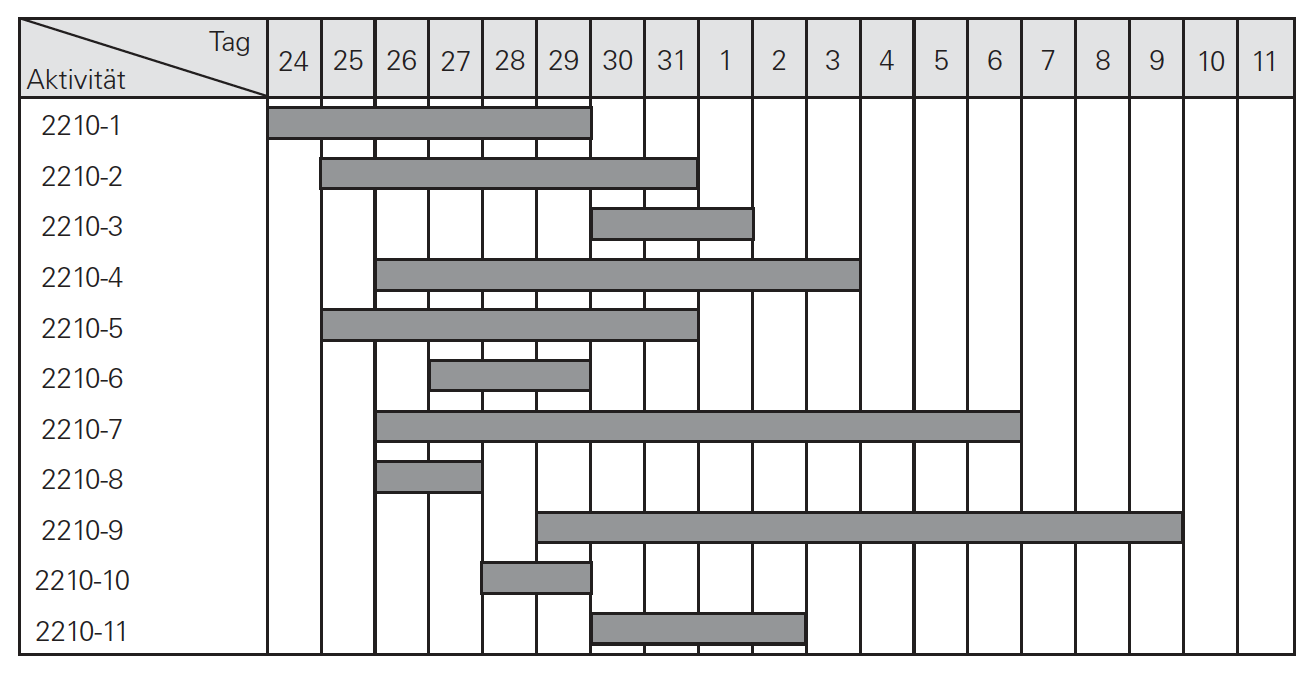
\includegraphics[width=15.323cm,height=7.856cm]{INMAusarbeitung02-img006.png}
\captionof{figure}[Beispiel eines Gantt{}-Diagramms]{Beispiel eines Gantt-Diagramms}
\label{seq:refIllustration5}
\par}
{\sffamily
Die Aktivitäten werden, wie das Beispiel zeigt, vertikal erfasst. Die horizontale Achse bildet den zeitlichen Ablauf ab.
Sie ist frei definierbare Zeiteinheiten, hier Tage, unterteilt. Den einzelnen Aktivitäten wurde in Abhängigkeit ihrer
Dauer ein jeweils entsprechend langer Balken zugeordnet. }


\bigskip

{\sffamily
Es gilt zu beachten, dass für jede Komponente die innerhalb des Projekts umgesetzt werden soll, ein solches Diagramm
erstellt wird. Damit wird der hohen Modularität des Projekts Rechnung getragen und eine entsprechend agile
Priorisierung der umzusetzenden Komponenten ist möglich. Die Reihenfolge der Umsetzung ist somit frei wählbar, ohne
dabei die Möglichkeit einer zeitlichen Planung bei der Umsetzung innerhalb Komponente zu verlieren.}

\subsubsection[Meilensteintrendanalyse]{\color{black} Meilensteintrendanalyse}
{\sffamily
Die Meilensteintrendanalyse (MTA) ist ein wichtiges und dabei einfach anzuwendendes Werkzeug zur Überwachung
essentieller Projekttermine. In diesem Zusammenhang werden Projekttermine auch Meileinsteine genannt. Die MTA liefert
dabei zwei grundlegende Informationen: Einerseits liefert sie einen Überblick über die Entwicklung zukünftiger Termine,
andererseits lässt sich anhand dieser Entwicklung die Stabilität der Terminprognosen erkennen\footnote{[GAD14]}.
\figurename~\ref{seq:refIllustration6} zeigt exemplarisch den Aufbau eines MTA-Diagramms.}


\bigskip

{\centering\sffamily
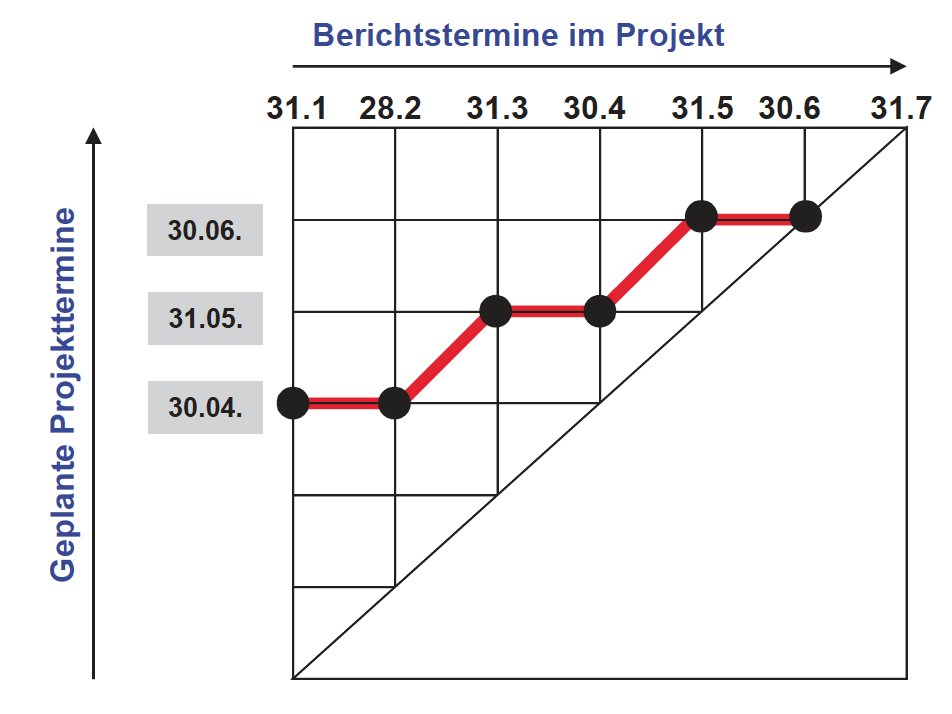
\includegraphics[width=9.225cm,height=6.92cm]{INMAusarbeitung02-img007.png}
\captionof{figure}[Aufteilung der Achsen der MTA]{Aufteilung der Achsen der MTA}
\label{seq:refIllustration6}
 \ 
\par}

{\sffamily
Wie in der Abbildung zu erkennen ist, besitzt ein MTA-Diagramm, wie auch das Gantt-Diagramm, zwei Dimensionen. Auf der
horizontalen Achse werden die Berichtstermine in vorher vereinbarten und regelmäßigen Abständen aufgetragen. Die
horizontale Achse ist mit den geplanten Projekterminen (Meilensteinen) beschriftet. Die Schnittstellen der Achsen geben
das aktuelle, möglicherweise korrigierte Fälligkeitsdatum des Meilensteins zum Zeitpunkt des Berichts an. In jedem
Bericht müssen die Meilensteintermine neu bewertet werden. Dabei ist es irrelevant ob der Temrin sich nach hinten
verschiebt, der Termin dem der letzten Beurteilung entspricht oder das geplante Datum unterschritten werden kann. Die
Ergebnisse dieser Beurteilungen werden in dem Diagramm eingetragen, woraus sich im Laufe des Projekts Kurven ergeben.
Diese Kurven entsprechen in der Regel einem der drei typischen Verläufe:}


\bigskip

\liststyleLSxvi
\begin{enumerate}
\item {\sffamily
Flache Kurve, entspricht dem Idealverlauf}
\item {\sffamily
Fallende Kurve, entspricht der Pessimistenschätzung}
\item {\sffamily
Steigende Kurve, entspricht dem Optimistenschätzung}
\end{enumerate}

\bigskip

{\sffamily
Eine fallende Kurve bedeutet, dass die ursprünglich geplanten Termine schneller erreicht wurden, während eine steigende
Kurve zeigt, dass die Termine entsprechend überschritten wurden.}


\bigskip

{\sffamily
Je kleiner der Intervall zwischen den Berichtsterminen gewählt wird, desto feiner ist die Granularität der
resultierenden Kurven, wodurch die Genauigkeit des Vergleichs zwischen ursprünglich geplanten Meilensteinterminen und
den während Projektausführung prognostizierten Terminen steigt\footnote{[GAD14]}. Die höhere Genauigkeit ermöglicht es,
kleinste Änderungen in dem ursprünglich geplanten Enddatum des Projekts zu registrieren, um entsprechend darauf
reagieren zu können. Nachfolgende Abbildungen \ref{seq:refIllustration7}, \ref{seq:refIllustration8},
\ref{seq:refIllustration9} stellen die gängigsten Kurvenverläufe einer MTA dar.}


\bigskip

{\centering 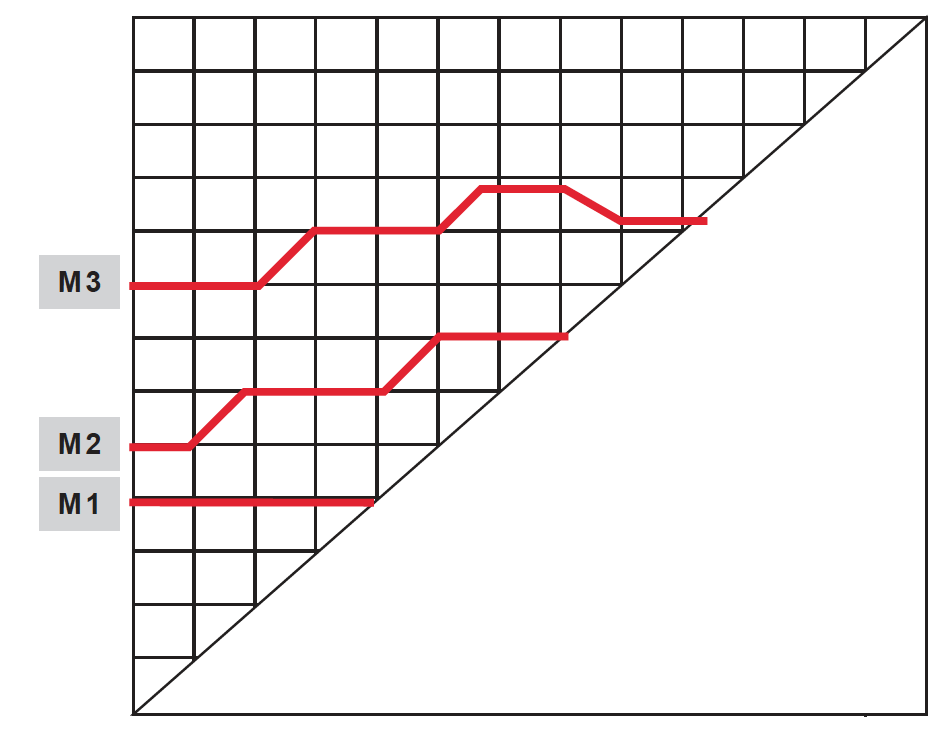
\includegraphics[width=8.881cm,height=6.944cm]{INMAusarbeitung02-img008.png}
\captionof{figure}[Idealverlauf der MTA{}-Kurven]{Idealverlauf der MTA-Kurven}
\label{seq:refIllustration7}
\par}
{\sffamily
\figurename~\ref{seq:refIllustration7} zeigt die Kurve des Idealverlaufs. Es ist zu erkennen, dass nur eine geringe
Anzahl an Korrekturen der Meilensteintermine nötig war. Die meisten Termine sind während der Projektausführung gleich
geblieben.}

{\centering 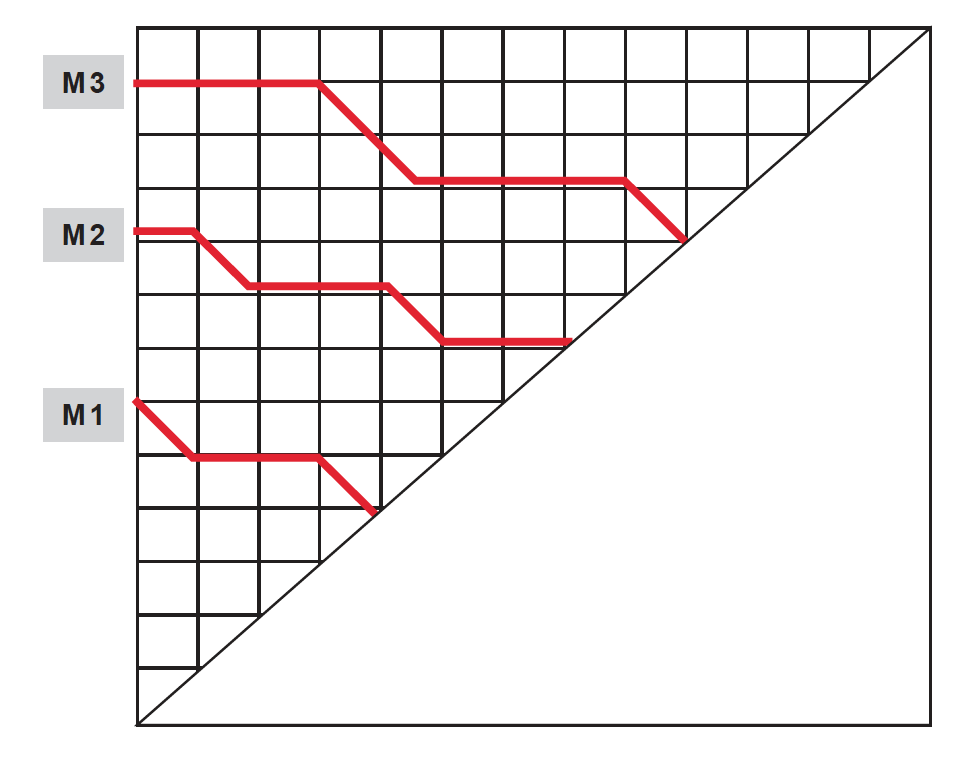
\includegraphics[width=8.902cm,height=7.177cm]{INMAusarbeitung02-img009.png}
\captionof{figure}[Kurvenverlauf der Pessimistenschätzung]{Kurvenverlauf der Pessimistenschätzung}
\label{seq:refIllustration8}
\par}
{\sffamily
Die fallenden Kurven in \figurename~\ref{seq:refIllustration8} zeigen, dass die Termine initial zu pessimistisch
geschätzt wurden und häufig nach unten korrigiert werden mussten. Eine Ursache hierfür können zu großzügig geplante
Puffer sein.}

{\centering 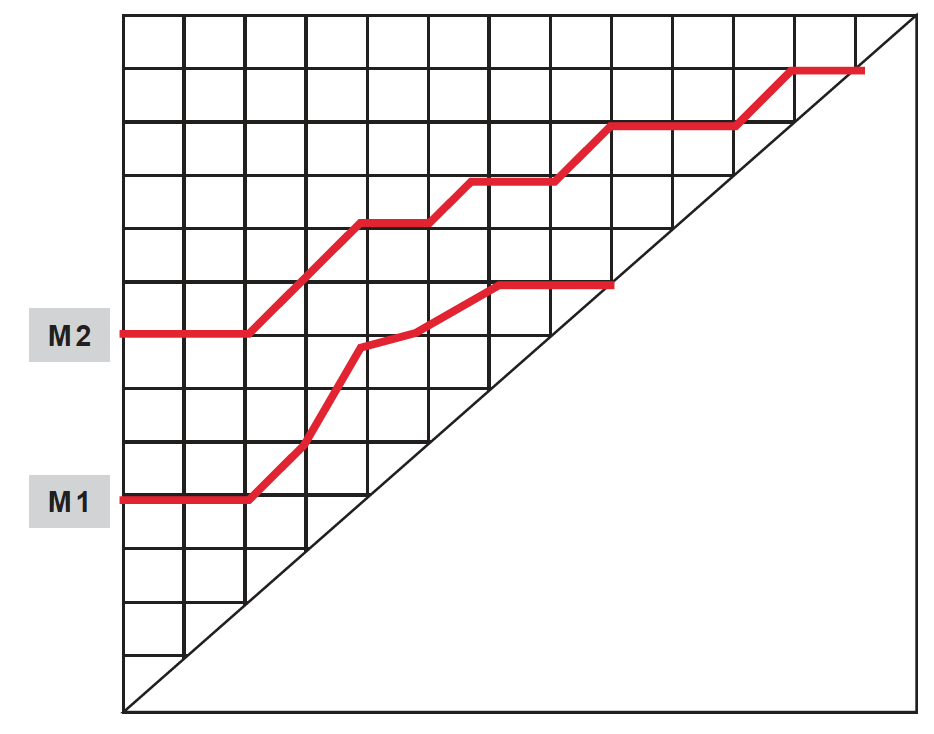
\includegraphics[width=9.091cm,height=7.158cm]{INMAusarbeitung02-img010.png}
\captionof{figure}[Kurvenverlauf der Optimistenschätzung]{Kurvenverlauf der Optimistenschätzung}
\label{seq:refIllustration9}
\par}
{\sffamily
Die in \figurename~\ref{seq:refIllustration9} gezeigte Kurve entspricht dem am häufigsten auftretenden Verlauf einer
Meileinsteinkurven. Die Termine werden nach hinten korrigiert wodurch der typische treppenartige Verlauf zustande
kommt. Ursachen hierfür können Fehleinschätzungen oder unerwartete Störungen sein\footnote{[GAD14]}.}

\subsection[Anwendung]{Anwendung}
{\sffamily
Nachdem die Werkzeuge zur zeitlichen und kostentechnischen Schätzung theoretisch beleuchtet wurden, werden diese im
Folgenden beispielhaft auf ausgewählte Komponenten des Projekts angewendet. Für die Einführung des
Dokumentenmanagementsystem Alfresco wird eine TCO-Analyse sowie ein Gantt-Diagramm angefertigt. Die potentiellen Kosten
des Redesigns der Hochschulwebseite (inkl. der Anpassung \ an moderne Ausgabegeräte) werden auf Grundlage von
Gesprächen mit entsprechenden Experten analysiert. Die Berechnungen des Zeitbedarfs geht davon aus, dass die
entsprechenden Komponenten des Projekts während des Semesters, also nicht zu besonders arbeitsintensiven Zeiten wie
Prüfungsphasen am Ende oder Planungsphasen am Anfang eines Semesters, durchgeführt werden.}

\subsubsection[Dokumentenmanagementsystem Alfresco]{\color{black} Dokumentenmanagementsystem Alfresco}
\label{bkm:RefHeading24767162299686}{\sffamily
Um erfolgreich ein Dokumentenmanagementsystem in einer Organisation einzuführen, müssen verschiedene Vorbedingungen
erfüllt sein. Das betrifft neben dem erforderlichen Personal zur Einrichtung, technischer Wartung, den Help-Desk und
inhaltlicher Pflege auch benötigte Hardware und Netzwerkinfrastruktur.}


\bigskip

{\sffamily
Um eine möglichst realitätsnahe Planung zu ermöglichen wurde hierzu Herr Stephan Voigt, aktuell CTO der Masterpayment
AG, befragt. Herr Voigt hat bereits zahlreiche CMS Projekte, unter anderem die Einführung von Alfresco als DMS bei der
Masterpayment AG, betreut, sodass seine Expertenmeinung verlässliche Zahlen ergibt. Diese Zahlen werden anschließend
anhand der beschriebenen TCO-Methode betrachtet. Die daraus resultierende \tablename~\ref{seq:refTable3} stellt einen
Überblick über die zu erwartenden Kosten dar. Folgende Bereiche wurden durch die Befragung beleuchtet:}

\liststyleLSxvii
\begin{itemize}
\item {\sffamily
Hardware für Anwenderprozesse und IT-Abteilung}
\item {\sffamily
Software für Anwenderprozesse, Help-Desk und Incidentmanagement}
\item {\sffamily
Prozessmanagement während des Betriebs durch Administartor(en)}
\item {\sffamily
Wartungsarbeiten durch Administrator(en)}
\item {\sffamily
Schulung der verantwortlichen Betreuer}
\item {\sffamily
Erstellen von Anwenderhandbuch}
\end{itemize}
{\sffamily
Da dies eine beispielhafte Betrachtung ist, geht die Berechnung davon aus, dass alle aufgeführten Ressourcen angeschafft
oder eingerichtet werden müssen. Sollte die Hochschule Teile dieser Ressourcen aus eigenem Bestand zur Verfügung
stellen, müssen die Werte in der TCO Berechnung entsprechend angepasst werden.}


\bigskip

\begin{table}
\centering
\begin{tabular}{|m{5.026cm}|m{6.3300004cm}|m{3.5449998cm}|}

\hline
{\sffamily\bfseries TCO-Kategorie} &
{\sffamily\bfseries Ressource/Tätigkeit} &
{\sffamily\bfseries Verbrauch}\\\hline
{\sffamily Hardware Anwender} &
{\sffamily Benötigte Hardware\newline
(Produktivsystem)} &
{\sffamily 4 Server, }

{\sffamily €\textrm{4.000 / Server}}\\\hline
{\sffamily Hardware Betreuer} &
{\sffamily Benötigte Hardware\newline
(Testsystem)} &
{\sffamily 2 Server,}

{\sffamily €\textrm{4.000/Server}}\\\hline
{\sffamily Software} &
{\sffamily Lizenzkosten} &
{\sffamily € \textrm{46.000}}

{\sffamily (2 x € 15.000\newline
Produktivsystem,}

{\sffamily 2 x € 3.500}

{\sffamily Testsystem,}

{\sffamily € \textrm{9.000 Clustering)}}\\\hline
{\sffamily Software Help-Desk/\newline
Incidentmanagement} &
{\sffamily Anschaffungs-/Lizenzkosten\newline
für Help-Desksoftwware} &
{\sffamily € \textrm{0,}}

{\sffamily Open Source}\\\hline
{\sffamily Prozessmanagement} &
{\sffamily Benutzer-/Systemverwaltung} &
{\sffamily 1 MT/Woche}\\\hline
{\sffamily Wartung des System} &
{\sffamily Backup der Datenbank, Updates} &
{\sffamily 1 MT/Woche}\\\hline
{\sffamily Schulung der\newline
Administratoren} &
{\sffamily Schulung durch Berater\newline
(Alfresco)} &
{\sffamily € \textrm{10000}}

{\sffamily (10 Tage,\newline
€ 1000/Tag)}\\\hline
{\sffamily Schulung der Mitarbeiter} &
{\sffamily Schulung durch Rechenzentrum} &
{\sffamily 2 MT}\\\hline
{\sffamily Erstellung von\newline
Anwenderhandbuch} &
{\sffamily Dokumentation für Anwender} &
{\sffamily 15 MT}\\\hline
{\sffamily Technischer Support} &
{\sffamily Help-Desk Tätigkeit} &
{\sffamily 1 Person, 2h/Tag}\\\hline\end{tabular}
\caption{Übersicht der Kosten für die TCO-Methode}
\label{seq:refTable3}
\end{table}

\bigskip

{\sffamily
Die in \tablename~\ref{seq:refTable3} erfassten Kosten werden in das, in Kapitel \ref{bkm:RefHeading24769162299686}
erwähnte, TCO-Tool übertragen. Anhand der verfügbaren Analysefunktionen werden anschließend die Gesamtkosten nach den
TCO-Kostenkategorien ausgegeben und aufgeschlüsselt. Das Ergebnis der Kalkulation anhand des TCO-Tools zeigt
\tablename~\ref{seq:refTable4}. \textcolor{black}{Die Betrachtung erfolgt dabei, entsprechend der Abschreibungsdauer
nach der
}DFG-Nutzungstabelle\footnote{https://www.physik.uni-muenchen.de/fakultaet/organisation/geschaeftsstelle/merkblaetter/dfg-tabelle.pdf},
üb\textcolor{black}{er einen Zeitraum von 48 Monaten.}}


\bigskip

\begin{flushleft}
\bottomcaption{Ergebnis der TCO-Methode}
\label{seq:refTable4}\tablefirsthead{}
\tablehead{}
\tabletail{}
\tablelasttail{}
\begin{supertabular}{|m{3.506cm}|m{1.9659998cm}|m{1.9659998cm}|m{1.9659998cm}|m{1.9659998cm}|m{2.931cm}|}
\hline
{\sffamily\bfseries\color{black} Kostenart } &
{\sffamily\bfseries\color{black} TCO\newline
1. Jahr } &
{\sffamily\bfseries\color{black} TCO\newline
2. Jahr } &
{\sffamily\bfseries\color{black} TCO\newline
3. Jahr } &
{\sffamily\bfseries\color{black} TCO\newline
4. Jahr } &
{\sffamily\bfseries\color{black} TCO-Kosten über gesamte Nutzungsdauer }\\\hline
{\sffamily\color{black} Datenbankmanagement } &
\raggedleft{\sffamily\color{black} 2.361,33 } &
\raggedleft{\sffamily\color{black} 2576} &
\raggedleft{\sffamily\color{black} 2.576,00 } &
\raggedleft{\sffamily\color{black} 2.576,00 } &
\raggedleft\arraybslash{\sffamily\color{black} 10.089,33 }\\\hline
{\sffamily\color{black} Hardware der\newline
IT-Abteilung} &
\raggedleft{\sffamily\color{black} 2.000,00 } &
\raggedleft{\sffamily\color{black} 2.000,00 } &
\raggedleft{\sffamily\color{black} 2.000,00 } &
\raggedleft{\sffamily\color{black} 2.000,00 } &
\raggedleft\arraybslash{\sffamily\color{black} 8.000,00 }\\\hline
{\sffamily\color{black} Hardware für Anwenderprozesse \ } &
\raggedleft{\sffamily\color{black} 6.250,00 } &
\raggedleft{\sffamily\color{black} 6.250,00 } &
\raggedleft{\sffamily\color{black} 6.250,00 } &
\raggedleft{\sffamily\color{black} 6.250,00 } &
\raggedleft\arraybslash{\sffamily\color{black} 25.000,00 }\\\hline
{\sffamily\color{black} Help Desk \ } &
\raggedleft{\sffamily\color{black} 13.135,50 } &
\raggedleft{\sffamily\color{black} 13.135,50 } &
\raggedleft{\sffamily\color{black} 13.135,50 } &
\raggedleft{\sffamily\color{black} 13.135,50 } &
\raggedleft\arraybslash{\sffamily\color{black} 52.542,00 }\\\hline
{\sffamily\color{black} Planungs- und Prozessmanagement } &
\raggedleft{\sffamily\color{black} 9.016,00 } &
\raggedleft{\sffamily\color{black} 9.016,00 } &
\raggedleft{\sffamily\color{black} 9.016,00 } &
\raggedleft{\sffamily\color{black} 9.016,00 } &
\raggedleft\arraybslash{\sffamily\color{black} 36.064,00 }\\\hline
{\sffamily\color{black} Schulung Endanwender } &
\raggedleft{\sffamily\color{black} 3.882,27 } &
\raggedleft{\sffamily\color{black} 0,00 } &
\raggedleft{\sffamily\color{black} 0,00 } &
\raggedleft{\sffamily\color{black} 0,00 } &
\raggedleft\arraybslash{\sffamily\color{black} 3.882,27 }\\\hline
{\sffamily\color{black} Schulung Mitarbeiter IT-Abteilung} &
\raggedleft{\sffamily\color{black} 2.500,00 } &
\raggedleft{\sffamily\color{black} 2.500,00 } &
\raggedleft{\sffamily\color{black} 2.500,00 } &
\raggedleft{\sffamily\color{black} 2.500,00 } &
\raggedleft\arraybslash{\sffamily\color{black} 10.000,00 }\\\hline
{\sffamily\color{black} Software der IT-Abteilung } &
\raggedleft{\sffamily\color{black} 1.750,00 } &
\raggedleft{\sffamily\color{black} 1.750,00 } &
\raggedleft{\sffamily\color{black} 1.750,00 } &
\raggedleft{\sffamily\color{black} 1.750,00 } &
\raggedleft\arraybslash{\sffamily\color{black} 7.000,00 }\\\hline
{\sffamily\color{black} Software für Anwenderprozesse} &
\raggedleft{\sffamily\color{black} 7.500,00 } &
\raggedleft{\sffamily\color{black} 7.500,00 } &
\raggedleft{\sffamily\color{black} 7.500,00 } &
\raggedleft{\sffamily\color{black} 7.500,00 } &
\raggedleft\arraybslash{\sffamily\color{black} 30.000,00 }\\\hline
{\sffamily\color{black} technischer Support } &
\raggedleft{\sffamily\color{black} 6.440,00 } &
\raggedleft{\sffamily\color{black} 6.440,00 } &
\raggedleft{\sffamily\color{black} 6.440,00 } &
\raggedleft{\sffamily\color{black} 6.440,00 } &
\raggedleft\arraybslash{\sffamily\color{black} 25.760,00 }\\\hline
{\sffamily\bfseries\color{black} Total } &
\raggedleft{\sffamily\bfseries\color{black} 54.835,10 } &
\raggedleft{\sffamily\bfseries\color{black} 51.167,50 } &
\raggedleft{\sffamily\bfseries\color{black} 51.167,50 } &
\raggedleft{\sffamily\bfseries\color{black} 51.167,50 } &
\raggedleft\arraybslash{\sffamily\bfseries\color{black} 208.337,60 }\\\hline
\end{supertabular}
\end{flushleft}

\bigskip

{\sffamily
\tablename~\ref{seq:refTable4} zeigt den finanziellen, beziehungsweise zeitlichen, Aufwand der nach Einschätzung des
befragten Experten nötig ist, um das Dokumentenmanagementsystem (DMS) Alfresco an der Hochschule einzuführen und zu
betreiben. Da in dem Interview mit dem Leiter des Rechenzentrums der Hochschule nicht geklärt werden konnte, in welchem
Rahmen dem Gesamtprojekt vorhandene Hardware zur Verfügung gestellt werden kann, wird in dieser TCO-Analyse davon
ausgegangen, dass Hardware angeschafft werden muss. }


\bigskip

{\sffamily
Aus Gründen der Hochverfügbarkeit wird Alfresco in einem Cluster betrieben. Dazu werden auf jeweils zwei Servern
Alfresco und eine dazugehörige Datenbank eingerichtet. Die Server mit einer entsprechend performanten Hardware liegen
bei €4.000 das Stück. Des Weiteren ist es ratsam, ein Testsystem zu installieren auf dem Updates oder zusätzliche
Eigenimplementierungen getestet werden können. Da ein solches Testsystem nicht der gleichen Last wie das
Produktivsystem ausgesetzt ist, ist es ausreichend zwei echte Server, auf denen jeweils zwei Server virtualisiert
werden, zu verwenden. Auch diese Server werden mit je € 4.000 veranschlagt.}


\bigskip

{\sffamily
Alfresco bietet von ihrer DMS-Software eine kostenfreie Community-Version und eine lizenzpflichtige Kauf-Version an. Das
größte Manko der Community-Version sind die nicht verfügbaren Aktualisierungen. Soll also eine bereits installierte
Community-Version auf eine neue Softwareversion aktualisiert werden, muss das gesamte System neu aufgesetzt werden. Der
Vorteil der regelmäßigen Aktualisierungen der kostenpflichtigen Version überwiegt also den Kostenvorteil der
kostenfreie Softwarelösung. }


\bigskip

{\sffamily
Die Lizenzgebühren für die Software liegen jeweils bei ca. € 15.000 für die Produktivsysteme und € 3.500 für die
Testsysteme. Dazu kommen Kosten in Höhe von ca. € 9.000 für Softwarekomponenten die den Betrieb im Cluster ermöglichen.
Da es zahlreiche Open-Source Lösungen für den Betrieb eines Help-Desks, beziehungsweise eines Ticketsystems, gibt,
fallen hierfür keine zusätzlichen Kosten an. }


\bigskip

{\sffamily
Nach der Installation läuft Alfresco zu einem großen Teil alleine und benötigt keine weitere Interaktion von außen. Es
fallen ledigliche kleinere Wartungsarbeiten, wie das Einspielen von Aktualisierungen oder das Anfertigen einer
Datenbanksicherung, an. Diese werden mit einem Aufwand von ca. 1 MT pro Woche veranschlagt. Dazu kommt die Verwaltung
der Benutzer des Systems mit einem weiteren MT pro Woche. Da die Mitarbeiter des Rechenzentrums hauptsächlich für den
Reibungslosen Betrieb der Plattform verantwortlich sein sollen, werden diese von Beratern der Alfresco Software AG
geschult. Die Schulung ist mit 10 Tagen geplant und verursacht Kosten in Höhe von € 1.000 je Tag. Anwender des Systems
können sich anschließend von den Mitarbeitern des Rechenzentrums schulen lassen. Für eine Anwenderschulung werden ca. 2
MT geplant. Zusätzlich wird ein Anwenderhandbuch erstellt. Die Erstellung dauert ca. 15 MT. Nach der Einführung des
System wird sich ein Mitarbeiter des Help-Desks erfahrungsgemäß etwa 2 Stunden täglich mit Anliegen rund um Alfresco
beschäftigen.}


\bigskip

{\sffamily
Die angenommenen Personalkosten entsprechen den Personalmittelsätzen für 2015 der DFG und beruhen auf
“Bruttoarbeitgeberkosten”. Die Grundlage der Berechnung der Stundensätze bildet die Anzahl der Arbeitstage des Jahres
2016 unter Berücksichtigung von, entsprechend den Tarifen des öffentlichen
Dienstes\footnote{http://oeffentlicher-dienst.info}, 30 Urlaubstagen und 39 Wochenstunden (insgesamt 224 Arbeitstage).
Die angenommenen Stundensätze sind zur Wahrung der Transparenz nachfolgend in \tablename~\ref{seq:refTable5}
dargestellt.}


\bigskip

\begin{center}
\bottomcaption{Übersicht der Jahres- und Stundenlöhne}
\label{seq:refTable5}\tablefirsthead{}
\tablehead{}
\tabletail{}
\tablelasttail{}
\begin{supertabular}{|m{8.792cm}|m{1.9359999cm}|m{2.432cm}|}
\hline
{\sffamily\bfseries\color{black} Personalkostenkategorie} &
{\sffamily\bfseries\color{black} EUR/Jahr} &
{\sffamily\bfseries\color{black} EUR/Stunde}\\\hline
{\sffamily\color{black} Postdoktorand/Postdokotrandin} &
\raggedleft{\sffamily\color{black} 65.400} &
\raggedleft\arraybslash{\sffamily\color{black} 37,50}\\\hline
{\sffamily\color{black} Doktorand/DoktorandIn} &
\raggedleft{\sffamily\color{black} 60.600} &
\raggedleft\arraybslash{\sffamily\color{black} 34,70}\\\hline
{\sffamily\color{black} Wissenschaftliche(r) Mitarbeiter/Mitarbeiterin} &
\raggedleft{\sffamily\color{black} 51.000} &
\raggedleft\arraybslash{\sffamily\color{black} 29,20}\\\hline
{\sffamily\color{black} Nichtwissenschaftlicher(r) Mitarbeiter/Mitarbeiterin} &
\raggedleft{\sffamily\color{black} 45.000} &
\raggedleft\arraybslash{\sffamily\color{black} 25,80}\\\hline
{\sffamily\color{black} Studentische Hilfskraft} &
~
 &
\raggedleft\arraybslash{\sffamily\color{black} 13,65}\\\hline
\end{supertabular}
\end{center}

\bigskip

{\sffamily
Der benötigte zeitliche Rahmen und der Ablauf der Einführung von Alfresco als Dokumentenmanagementsystems wird durch ein
Gantt-Diagramm visualisiert. Die Daten für die Erstellung dieses Diagramms wurden ebenfalls im Rahmen der
Expertenbefragung ermittelt.}

{\sffamily
\textrm{Das Gantt-Diagramm in \figurename~\ref{seq:refIllustration10} zeigt die Dauer der einzelnen Teilschritte der
Einführung des Teilprojektes „Alfresco“. Die Gesamtdauer des Teilprojekts ist die Strecke zwischen dem Anfang des
obersten und dem Ende des untersten Balkens. Die Datumsangaben sind hier zu ignorieren, es geht nur um die Gesamtzahl
an Manntagen, die die Umsetzung des Teilprojekts benötigt. Im ersten Schritt müssen die Server sowohl für Test- als
auch für die Produktivsysteme konfiguriert und in das vorhandene Netzwerk integriert werden. Danach wird die Software
installiert und entsprechend den Vorgaben der Fachbereiche konfiguriert. Nach der Installation können die
Administratoren des DMS geschult werden um in dem nächsten Schritt ein Handbuch erstellen zu können. Die
Qualitätsicherung des Handbuches und des DMS folgt zum Abschluss des Projekts. Ingesamt dauert die Einführung 30 MT.} }

\begin{figure}
\centering
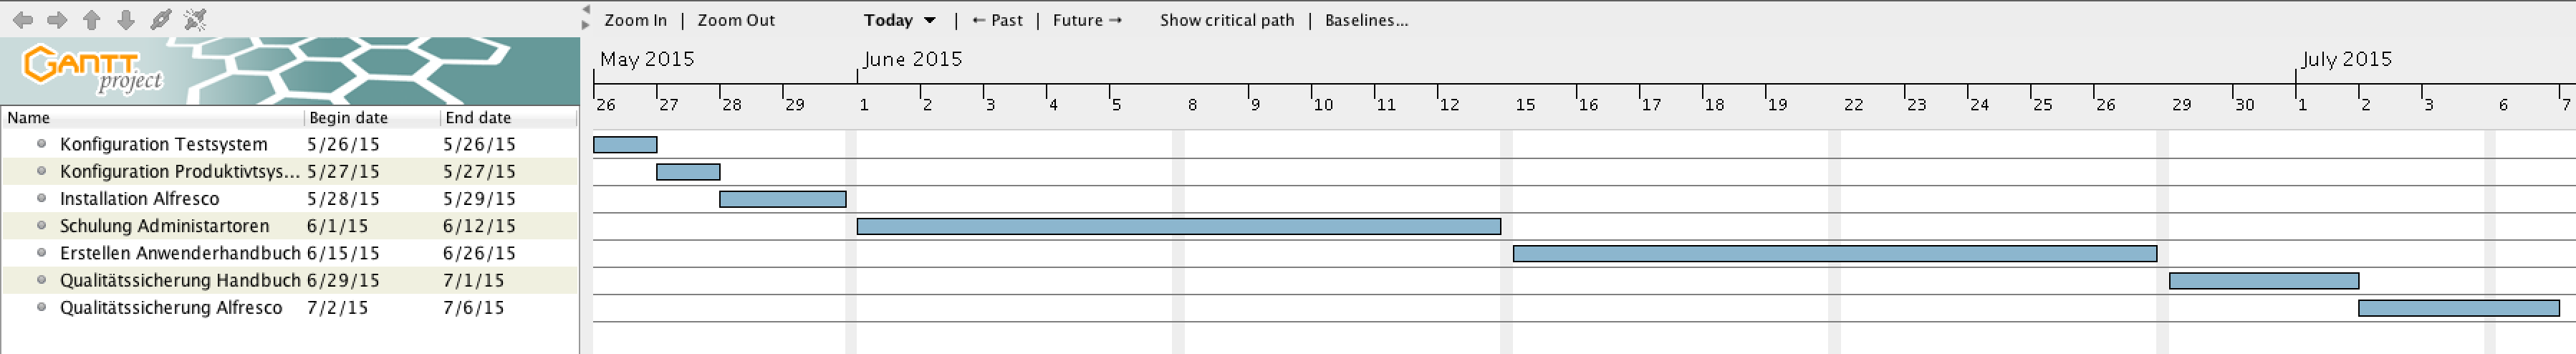
\includegraphics[width=15.501cm,height=2.129cm]{INMAusarbeitung02-img011.png}
\caption[Gantt Diagramm Alfresco]{Gantt Diagramm Alfresco}
\label{seq:refIllustration10}

\end{figure}
\subsubsection[Redesign/Relaunch Hochschul{}-Webseite]{\color{black} Redesign/Relaunch Hochschul-Webseite}
\label{bkm:RefHeading24771162299686}{\sffamily
Um den Aufwand - und damit auch den Kosten- und Zeitrahmen der Umsetzung einer neuen Hochschulwebsite zu ermitteln,
wurden Gespräche mit mehreren Experten\footnote{Achim Gosse, Geschäftsführender Gesellschafter digitalnoise GmbH
(www.digitalnoise.de/)}\textsuperscript{;}\footnote{Stefan Becker, Software- und Webentwickler (www.beckeste.de)}
geführt. Die Ergebnisse dieser Gespräche finden sich zuammengefasst in \tablename~\ref{seq:refTable6}\textcolor{blue}{,
}welche\textcolor{blue}{ }die verschiedenen Phasen des Entwicklungsprozesses, vom initialen Workshop bis hin zur
Auslieferung und Qualitätsicherung, abbildet. Als Einheit wird dabei auf “Manntage” (MT) statt auf monetäre Angaben
gesetzt, da Stunden- und Tagessätze teils starken regionalen Unterschieden unterliegen. Es gilt zu beachten, dass die
hier durchgeführte Betrachtung der Kosten lediglich die externen Kosten berücksichtigt. Ausfallzeiten von Mitarbeitern,
die beispielsweise durch die Teilnahme an Workshops generiert werden, werden nicht berücksichtigt.}


\bigskip

\begin{center}
\bottomcaption{Aufwandsschätzung zum Redesign der Hochschul-Website}
\label{seq:refTable6}\tablefirsthead{}
\tablehead{}
\tabletail{}
\tablelasttail{}
\begin{supertabular}{|m{4.497cm}|m{2.1829998cm}|}
\hline
{\sffamily\bfseries\color{black} Aufgabe} &
{\sffamily\bfseries\color{black} Manntage}\\\hline
{\sffamily\color{black} Workshop} &
\raggedleft\arraybslash{\sffamily\color{black} 5}\\\hline
{\sffamily\color{black} Konzept} &
\raggedleft\arraybslash{\sffamily\color{black} 10}\\\hline
{\sffamily\color{black} Präsentation Konzept} &
\raggedleft\arraybslash{\sffamily\color{black} 2}\\\hline
{\sffamily\color{black} User Experience} &
\raggedleft\arraybslash{\sffamily\color{black} 5}\\\hline
{\sffamily\color{black} Design} &
\raggedleft\arraybslash{\sffamily\color{black} 15}\\\hline
{\sffamily\color{black} Präsentation Design} &
\raggedleft\arraybslash{\sffamily\color{black} 2}\\\hline
{\sffamily\color{black} Endpräsentation } &
\raggedleft\arraybslash{\sffamily\color{black} 3}\\\hline
{\sffamily\color{black} technische Umsetzung} &
\raggedleft\arraybslash{\sffamily\color{black} 2}\\\hline
{\sffamily\color{black} Anpassung Content} &
\raggedleft\arraybslash{\sffamily\color{black} 5}\\\hline
{\sffamily\color{black} Qualitätssicherung} &
\raggedleft\arraybslash{\sffamily\color{black} 3}\\\hline
{\sffamily\color{black} Deployment} &
\raggedleft\arraybslash{\sffamily\color{black} 1}\\\hline
{\sffamily\color{black} Puffer} &
\raggedleft\arraybslash{\sffamily\color{black} 5}\\\hline
{\sffamily\color{black} Gesamt} &
\raggedleft\arraybslash{\sffamily\color{black} 48 - 53}\\\hline
\end{supertabular}
\end{center}

\bigskip

{\sffamily
Der Initiale Schritt des gesamten Prozesses sollte, sofern im Voraus kein ausgearbeitetes Konzept vorliegt, in der
Durchführung von Workshops mit Entscheidungsträgern aus allen beteiligten Bereichen (Verwaltung, Fachbereiche,
Rechenzentrum, etc.) liegen. Um das Ziel des Workshops, nämlich eine gemeinsame Grundlage zu schaffen, die von allen
gleichermaßen getragen wird, zu erreichen, werden, bedingt durch das vorhandene Konfliktpotential, 5 Manntage zur
Durchführung angesetzt.}


\bigskip

{\sffamily
Die Ergebnisse des Workshops werden anschließend durch Konzeptioner, die an dem Workshop als “Zuhörer” teilgenommen
haben, verarbeitet, um daraus ein Website-Konzept zu entwickeln. Für die Ausarbeitung des Konzepts mit entsprechender
Präsentation vor den Projektverantwortlichen der Hochschule werden 12 Manntage veranschlagt.}


\bigskip

{\sffamily
Nachdem das Konzept freigegeben wurde, können User-Experience-Experten und (User Interface-)Designer mit der
Ausarbeitung der Gestaltungsvorlage beginnen. Dabei ist es üblich, dem Kunden mehrere, möglichst unterschiedliche,
Designvorschläge zu unterbreiten. Inklusive Präsentation und Ausarbeitung des finalen Vorschlags kann dieser Posten mit
22 Manntagen berechnet werden.}


\bigskip

{\sffamily
Auf Basis des verabschiedeten Designs kann die technische Realisierung der neuen Konzepte und Gestaltungsvorlagen
beginnen. Da zum einen die benötigten Kompetenzen innerhalb der Hochschule vorhanden sind und zum anderen das interne
Konfliktpotential in diesem Schritt wesentlich geringer ausfällt, bietet es sich an, diesen Schritt hochschulintern
durchzuführen. Die kalkulierten 7 Manntage durch die Dienstleister setzen sich aus den Punkten “technische Umsetzung”
(2 Manntage) und “Anpassung Content” (5 Manntage) zusammen. Die 2 Mantage der techniscnhe Umsetzung sind dabei zur
Unterstützung des Hochschulteams vorgesehen, während die 5 Tage vor allem genutzt werden, um auf “content-seitige”
Sonderfälle reagieren zu können. Da bereits TYPO3 als Content Management System zum Einsatz kommt, sollte die Migration
des bestehenden Inhalts in ein neues System entfallen. Durch die Möglichkeit des Multi-Channel-Publishings und
Hilfsmittel zur Erstellung barrierearmer Websites ist ein Wechsel des Systems nicht erforderlich.}


\bigskip

{\sffamily
Vor der Auslieferung und dem “live gehen” des Internetauftritts steht noch die finale Qualitätssicherung. Dabei wird die
gesamte Webpräsenz abschließend auf Konsistenz und Fehlerfreiheit geprüft. Bei einer Website diesen Umfangs werden für
die Überprüfung und Korektur eventueller Fehler 3 Manntage berechnet.}


\bigskip

{\sffamily
Die eigentliche Auslieferung sollte nach der Qualitätssicherung innerhalb eines Arbeitstages durchgeführt sein. Zur
Absicherung wird eine Arbeitswoche als Puffer veranschlagt, sodass die Umsetzung des Projekts im Kostenrahmen von 48
bis 53 Manntagen liegt.}


\bigskip

{\sffamily\color{black}
Da das Erstellen eines Konzepts für einen komplexen Internetauftritt im Allgemeinen mit einem nicht zu unterschätzenden
Aufwand verbunden ist, wird ein solches Konzept durch die entsprechenden Agenturen in der Regel nur angefertigt, wenn
dahinter die Aussicht auf den Erhalt des entsprechenden Auftrags steht. Da weder ein bestehendes Konzept, noch die
konkrete Aussicht auf einen tatsächlichen Auftrag vorliegen, konnten durch die Dienstleister keine konkreten Angebote
abgegeben werden.}

\subsubsection[Facebook Seite]{\color{black} Facebook Seite}
{\sffamily
Facebook unterscheidet verschiedene Arten von Applikationen die mit einem Profil verknüpft werden können. Dabei ist es
unerheblich ob dieses Profil einer Privatperson, einem Unternehmen oder einer anderen Organisation zugeordnet
wird\footnote{https://developers.facebook.com/docs}.}


\bigskip

{\sffamily
Die Hochschule Emden/Leer hat bereits ein reguläres Facebook Profil. Es gilt nun für die einzelnen Fachbereiche
sogenannte “Page Tabs” einzurichten. “Page Tabs” werden auf einer Facebook Profil-Seite als Menü-Links eingeblendet.
Der Inhalt der Tabs wird wird mit einer, nach speziellen Vorgaben gestalteten, Webseite in die Profil-Seite integriert.
Facebook gibt mit einer API das Format vor. Auch die Nutzung anderer Elemente der Facebook Dienste bedarf einer
Integration der Facebook API. Dabei ist zu beachten, dass die Webseite, deren Inhalt in dem Tab angezeigt wird, auf
einem externen Server, in diesem Fall einem Server der Hochschule,
liegt\footnote{https://developers.facebook.com/docs}.}


\bigskip

{\sffamily
Bei der Ermittlung des Zeitbedarfs für die Erstellung eines Tabs geht es folglich darum, den zeitlichen Aufwand für das
Anfertigen einer regulären Webseite nach den Vorgaben der Facebook API zu schätzen. Die benötigten Funktionen einer
solchen Webseite und der dazugehörige Entwicklungsaufwand werden wieder durch Befragung eines Experten ermittelt. Als
Experte für dieses Teilprojekt stand Herr Dipl.-Inf. Franz Riehl von der jambit GmbH aus München zur Verfügung. Analog
zur Kalkulation der Website in Kapitel \ref{bkm:RefHeading24771162299686} wird auch in diesem Fall in “Manntagen”
gerechnet:}


\bigskip

\begin{center}
\bottomcaption{Aufwandsschätzung zur Entwicklung der {\textquotedbl}Facebook Page Tabs{\textquotedbl}}
\tablefirsthead{}
\tablehead{}
\tabletail{}
\tablelasttail{}
\begin{supertabular}{|m{2.744cm}|m{2.247cm}|}
\hline
{\sffamily\bfseries\color{black} Aufgabe} &
{\sffamily\bfseries\color{black} Manntage}\\\hline
{\sffamily\color{black} Konzept} &
{\sffamily\color{black} 1 }\\\hline
{\sffamily\color{black} Design} &
{\sffamily\color{black} 10 }\\\hline
{\sffamily\color{black} Präsentation} &
{\sffamily\color{black} 1 }\\\hline
{\sffamily\color{black} Realisierung} &
{\sffamily\color{black} 8 }\\\hline
{\sffamily\color{black} Integration} &
{\sffamily\color{black} 1}\\\hline
{\sffamily\color{black} Abnahme/QS} &
{\sffamily\color{black} 1}\\\hline
{\sffamily\color{black} Summe} &
{\sffamily\color{black} 22 }\\\hline
\end{supertabular}
\end{center}

\bigskip

{\sffamily
Der initiale Schritt besteht erneut in der Konzeption der einzubindenden Webanwendung. Da das Konzept der Page-Tabs für
jeden Fachbereich identisch sein sollte, fällt der konzeptionelle Aufwand nur einmalig an. Das Konzept besteht in
diesem Fall aus der Auswahl der zu transportierenden Informationen und einer entsprechenden Darstellungsform, wofür 1
Manntag kalkuliert wird.}


\bigskip

{\sffamily
Im Gegensatz zum Konzept sollte die Gestaltung der Page-Tabs an den jeweiligen Fachbereich angepasst werden. Da es im
Idealfall bereits ein Corporate-Design Manual gibt, in dem grundlegende Gestaltungsrichtlinien festgehalten sind,
werden für diesen Schritt 2,5 Tage pro Fachbereich berechnet, sodass in Summe 10 Manntage berücksichtigt werden
müssen.}


\bigskip

{\sffamily
Nach der Präsentation aller vier Designs, wofür 1 Manntag veranschlagt wird, folgt die Realisierung. Da die Gestaltung
an die Fachbereiche angepasst wurde, können die Vorlagen voraussichtlich nicht alle nach dem gleichen Schema umgesetzt
werden, weshalb für jeden Page-Tab 2 Manntage kalkuliert werden.}


\bigskip

{\sffamily
Die finalen Schritte bestehen in der Facebook-Integration mit abschließender Qualitätssicherung. Pro Fachbereich kann
diesbezüglich ein halber Manntag vorgesehen werden, sodass die letzten Punkte mit insgesamt 2 Manntagen zu Buche
schlagen. Die Gesamtsumme beträgt bei dem beschriebenen Vorgehen 22 Manntage.}


\bigskip

{\sffamily
Da es sich bei dem Facebook-Auftritt nicht um ein “kritisches System” im Sinne der Verfügbarkeit der Anwendung handelt,
bietet es sich an, die Webanwendungen im Rahmen einer Projekt- oder Bachelorarbeit umsetzen zu lassen. Neben der
Tatsache, dass so die Gestaltung und Umsetzung “direkt durch die Zielgruppe” des Auftritts geschieht, können dadurch
Kosten eingespart werden. Alternativ sollte auf studentische Hilfskräfte zurückgegriffen werden.}


\bigskip

{\sffamily
Eine exemplarische Kalkulation auf Grundlage der bereits in Kapitel \ref{bkm:RefHeading24767162299686} erfassten
Stundensätze zeigt \tablename~\ref{seq:refTable8}.}


\bigskip

\begin{table}
\centering
\begin{tabular}{|m{2.9099998cm}|m{2.247cm}|m{6.316cm}|m{1.791cm}|}

\hline
{\sffamily\bfseries\color{black} Aufgabe} &
{\sffamily\bfseries\color{black} Manntage} &
{\sffamily\bfseries\color{black} Personalkostenkategorie} &
{\sffamily\bfseries\color{black} Betrag}\\\hline
{\sffamily\color{black} Konzept} &
\raggedleft{\sffamily\color{black} 1} &
{\sffamily\color{black} studentische Hilfskraft} &
\raggedleft\arraybslash{\sffamily\color{black} 13,65}\\\hline
{\sffamily\color{black} Design} &
\raggedleft{\sffamily\color{black} 10} &
{\sffamily\color{black} studentische Hilfskraft} &
\raggedleft\arraybslash{\sffamily\color{black} 136,50}\\\hline
{\sffamily\color{black} Präsentation} &
\raggedleft{\sffamily\color{black} 0,5\newline
0,5} &
{\sffamily\color{black} studentische Hilfskraft\newline
Nichtwissenschaftlicher Mitarbeiter} &
\raggedleft\arraybslash{\sffamily\color{black} 6,83\newline
12,90}\\\hline
{\sffamily\color{black} Realisierung} &
\raggedleft{\sffamily\color{black} 8} &
{\sffamily\color{black} studentische Hilfskraft} &
\raggedleft\arraybslash{\sffamily\color{black} 109,20}\\\hline
{\sffamily\color{black} Integration} &
\raggedleft{\sffamily\color{black} 1} &
{\sffamily\color{black} studentische Hilfskraft} &
\raggedleft\arraybslash{\sffamily\color{black} 13,65}\\\hline
{\sffamily\color{black} Abnahme/QS} &
\raggedleft{\sffamily\color{black} 1} &
{\sffamily\color{black} Nichtwissenschaftlicher Mitarbeiter} &
\raggedleft\arraybslash{\sffamily\color{black} 25,80}\\\hline
{\sffamily\color{black} Summe} &
\raggedleft{\sffamily\color{black} 21,5} &
~
 &
\raggedleft\arraybslash{\sffamily\color{black} 318,53}\\\hline\end{tabular}
\caption{Exemplarische Kostenkalkulation der Umsetzung der {\textquotedbl}Facebook Page Tabs{\textquotedbl}}
\label{seq:refTable8}
\end{table}

\bigskip

{\sffamily
Die Realisierung der Page-Tabs durch eine studentische Hilfskraft würde folglich ca. 350 Euro kosten. Da die
Präsentation vermutlich vor einem nichtwissenschaftlichen Mitarbeiter gehalten wird, müssen auch dessen Personalkosten
für den Zeitraum der Präsentation berücksichtigt werden. Ebenso erfolgt die Abnahme und Qualitätssicherung
voraussichtlich durch einen nichtwissenschaftlichen Mitarbeiter.}

\clearpage\setcounter{page}{1}\pagestyle{Standard}
\section{Ausgewählte Projekt-Beispiele}
\label{bkm:RefHeading24761162299686}{\sffamily
Die DFG hatte im Bezug auf die Förderung in jedem Durchgang die vier besten Projekte ausgewählt. Diese wurden mit 50.000
€ für die detaillierte Planungsphase und deren Umsetzung ausgestattet. In einem zweiten Förderzeitraum, von maximal 5
Jahren, wurden zwei der vier Projekte mit jeweils 250.000 €~pro Jahr ausgestattet.\textcolor{red}{ }Insgesamt
entspricht das einem Fördervolumen von gut 1,3 Mio. € für ein integriertes Informationsmanagement. Die folgenden
Projekte wurden im Zeitraum 2005 - 2010 durchgeführt und haben ihre Erfahrungen in Publikationen
bereitgestellt\footnote{[KER05]}.}


\bigskip

{\sffamily
Als Bestätigung dieser Zahlen weist die TU München mehr als f\"{u}nfzig Mitarbeiterinnen und Mitarbeiter im Projekt aus.
Zu ihrem integrierten Informationsmanagement bekam das Projekt insgesamt ca. 2,5 Mio. €. Die TU M\"{u}nchen stellte
dazu selbst weitere Sondermittel aus dem Erneuerungsprojekt InnovaTUM zur Verf\"{u}gung\footnote{[BOD10]}.}

\subsection{Beispiele des integrierten Informationsmanagements}
{\sffamily
Münster Information System for Research and Organization (MIRO) ist das integrierte Informationsmanagement an der
Westfälischen Wilhelms-Universität \ (WWU) Münster. }


\bigskip

{\sffamily
Die ersten Bemühungen starteten im Jahr 2003 und wurden in den folgenden Jahren vorangetrieben. Im Jahre 2005 wie zum
abschließenden Berichtsstand der WWU 2013 existierten 15 Fachbereiche an der WWU. Die 130 Studienfächer sanken in
diesem Zeitraum auf 110. Auch die ca. 39.000 Studierenden sind im Jahr 2013 auf ca. 37.000 Studierende gesunken. An der
WWU waren zum Zeitpunkt der Antragstellung etwa 5.000 Personen beschäftigt, davon 600 Professoren, 2.600
wissenschaftliche und 1.800 weitere Mitarbeiter. Im Jahr 2013 sind über 550 Professoren und ca. 3800 wissenschaftliche
Beschäftigte an der WWU\footnote{[VOG13]}.\newline
}

\liststyleLSxviii
\begin{itemize}
\item {\sffamily
Erreichtes}

\begin{itemize}
\item {\sffamily
Flexible IT-Architektur – SOA / SOI\ \ \ \ }
\item {\sffamily
Identitätsmanagement (MORITZ)\ \ \ \ }
\item {\sffamily
Digitales Publizieren\ \ \ \ }
\item {\sffamily
Enterprise Content Management (ECM) (Alfresco, SAN, Oracle Cluster)\ \ }
\item {\sffamily
Mobile Dienste (Alfresco)\ \ }
\item {\sffamily
Portalinfrastruktur (Apache Webserver, JBoss Portal, Oracle Cluster)\ \ \ \ }
\end{itemize}
\item {\sffamily
Aufwand\ \ }

\begin{itemize}
\item {\sffamily
16 wissenschaftlichen Mitarbeiterstellen - 8 davon DFG gefördert\ \ }
\item {\sffamily
\"{u}ber einen Zeitraum von sechs Jahren}
\item {\sffamily
Finanzmittel\ \ \ \ }

\begin{itemize}
\item {\sffamily
beträchtliche Finanzmittel durch das Rektorat der Universität}
\item {\sffamily
vor allem notwendige Sachausgaben}
\end{itemize}
\end{itemize}
\end{itemize}

\bigskip

{\sffamily
„\textit{Nach über zehn Jahren ist festzuhalten, dass sich die Strukturen in der Informa- tionsverarbeitung und
-versorgung sehr bewährt haben. Den Verantwortlichen ist es gelungen, die Informationsverarbeitung und -versorgung in
Münster auf einen beachtlichen Stand der Technik und Organisation zu bringen.}“\footnote{[BOD10]}}


\bigskip

\begin{center}
\bottomcaption{Annahme der minimalen Investition in Münster}
\label{seq:refTable9}\tablefirsthead{}
\tablehead{}
\tabletail{}
\tablelasttail{}
\begin{supertabular}{|m{7.046cm}|m{5.063cm}|}
\hline
{\sffamily\bfseries\color{black} Kostenaufteilung Annahme MIRO} &
{\sffamily\bfseries\color{black} Betrag in €}\\\hline
{\sffamily\color{black} Gesamtvolumen über 5 Jahre (bekannt)} &
{\sffamily\color{black} 1.300.000}\\\hline
{\sffamily\color{black} Personalkosten IT ca. 75 \%} &
{\sffamily\color{black} 975.000}\\\hline
{\sffamily\color{black} Kosten pro Projektmitarbeiter (16)} &
{\sffamily\color{black} 56.875 \ ( ca. 5080 / Monat )}\\\hline
{\sffamily\color{black} Sonstige Kosten ( unbekannt )} &
{\sffamily\color{black} 325.000 ( ca. 65.000 / Jahr )}\\\hline
\end{supertabular}
\end{center}
{\sffamily
Die geschätzten Kosten der Projektmitarbeiter der \tablename~\ref{seq:refTable9} passen zu den Angaben der DFG-Sätze
2015, worin ein/e Doktorandin/ Doktorand und Vergleichbare 5.050 € monatlich verdienen und Sonstige(r)
wissenschaftliche(r) Mitarbeiterinnen oder Mitarbeiter 4.250 € Vergütung erhalten (vgl. \tablename~\ref{seq:refTable5})
. Das Mittel von der Professur Vergütung bis zum angestellten Mitarbeiter liegt sogar etwas höher bei ca. 5240 €
monatliche Vergütung\textcolor{red}{.}}


\bigskip

{\sffamily
Die Angabe der Personalkosten von 75 \% \ leitet sich aus einem Bericht der Kosten in fertigenden Unternehmen und der
Automobilbranche ab\footnote{[SCH09]}. }


\bigskip

{\sffamily
Ein weiteres Projekt ist das „Karlsruher Integriertes InformationsManagement“ (KIM).}

{\centering 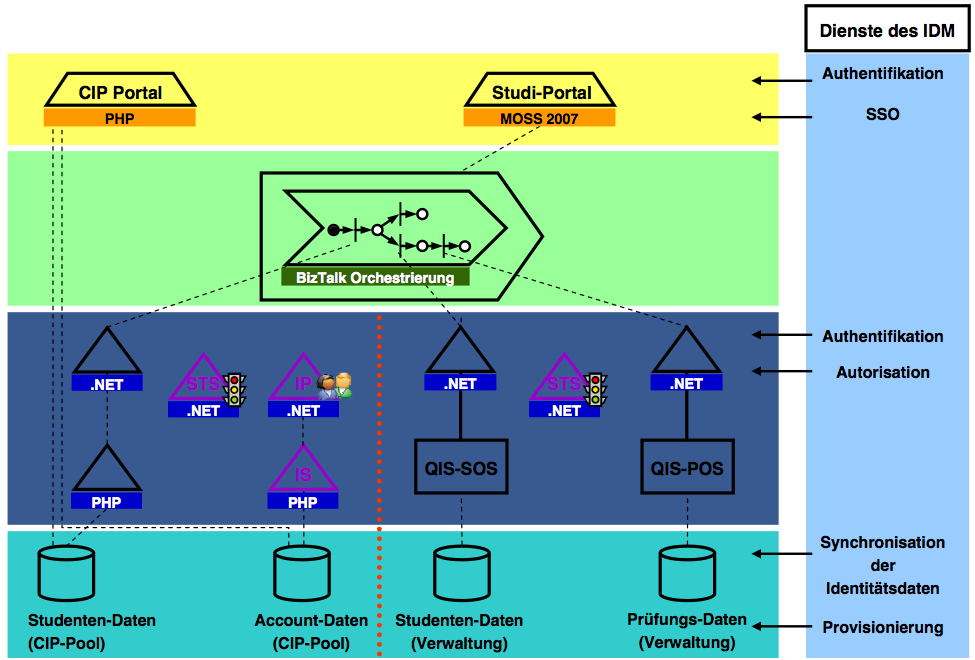
\includegraphics[width=15.404cm,height=10.433cm]{INMAusarbeitung02-img012.png}
\captionof{figure}[Erreichtes im Überblick für Karlsruhe (Juling Best Practice Workshop 2008)]{Erreichtes im Überblick
für Karlsruhe \textcolor[rgb]{1.0,0.2,0.2}{(}\textcolor{red}{Juling Best Practice Workshop 2008)}}
\par}
{\sffamily
KIM ist im Ansatz eine dienstorientierte F\"{o}deration, in der die jeweiligen Fachbereiche sich an bestimmte
Schnittstellen halten und selbst die Dienste in ihrer bevorzugten Art und Programmierung zur Verfügung stellen. Dabei
wurde ein hoch komplexes, aber nach eigenen Angaben sehr flexibles System, im Rahmen der 5 Jahre DFG Förderung,
geschaffen\footnote{[BOD10]}.}


\bigskip

{\sffamily
An der Universität Karlsruhe studieren (Stand 02/2014) ca. 24.500 Studenten ca. 9500 Mitarbeiter davon 346 Professoren
mit Einnahmen in Mio. € 795 wovon Drittmittel 339 Mio. € betragen. Die Landesmittel sind mit 212 Mio. € und die
Bundesmittel mit 349 Mio. € angegeben\footnote{https://www.kit.edu/mediathek/print\_forschung/Flyer\_KIT\_de.pdf}. Den
CIO bilden Rektorat und Vorstand.}

{\centering 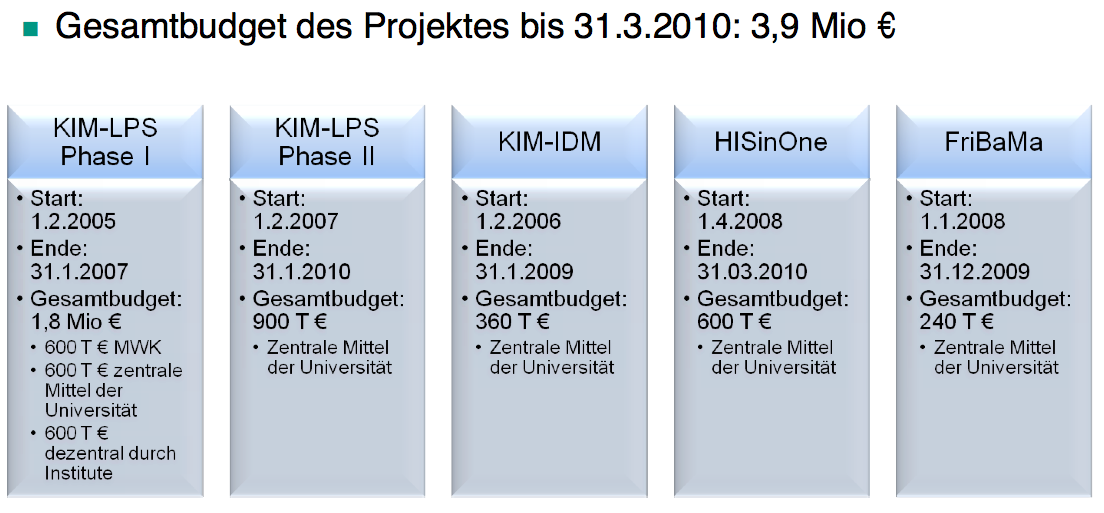
\includegraphics[width=15.425cm,height=7.153cm]{INMAusarbeitung02-img013.png}
\captionof{figure}[Überblick zum Projekt{}-Budget KIM (Juling Best Practice Workshop 2008)]{Überblick zum Projekt-Budget
KIM \textcolor[rgb]{1.0,0.2,0.2}{(}\textcolor{red}{Juling Best Practice Workshop 2008)}}
\par}
{\sffamily
Aus den bekannten Werten des Projektes MIRO kann nun abgeleitet werden, wieviele Personen an dem Projekt mitgewirkt
haben könnten und welche Beträge für sonstige Kosten zur Verfügung standen. Diese Annahme in der
\textcolor[rgb]{0.6,0.0,1.0}{\tablename~\ref{seq:refTable10}} ist rein fiktiv und dient lediglich dem Vergleich mit dem
Projekt MIRO, dass den selben DFG-Förderungen gegenüber steht.}


\bigskip

\begin{table}
\centering
\begin{tabular}{|m{7.4550004cm}|m{5.065cm}|}

\hline
{\sffamily\bfseries\color{black} Kostenaufteilung Annahme KIM} &
{\sffamily\bfseries\color{black} Betrag in €}\\\hline
{\sffamily\color{black} Gesamtvolumen über 5 Jahre (bekannt)} &
{\sffamily\color{black} 3.900.000}\\\hline
{\sffamily\color{black} Personalkosten IT ca. 75 \%} &
{\sffamily\color{black} 2.925.000}\\\hline
{\sffamily\color{black} Kosten pro Projektmitarbeiter (50 möglich)} &
{\sffamily\color{black} 58.500 ( ca. 4875 / Monat )}\\\hline
{\sffamily\color{black} Sonstige Kosten ( unbekannt )} &
{\sffamily\color{black} 975.000 ( ca. 81.250 / Jahr )}\\\hline\end{tabular}
\caption{Annahme der minimalen Investition in Karlsruhe}
\label{seq:refTable10}
\end{table}

\bigskip

{\sffamily
Die Hochschule Emden/Leer ist mit 4.626 Studierenden eine kleine Hochschule, für die nun in
\tablename~\ref{seq:refTable11} beispielhaft eine fiktive Annahme durch Teilung, aus den Werten des MIRO Projektes,
gezeigt wird. Die Grundlage wäre das Minimum, dass dem MIRO Projekt durch seine DFG Förderung zukam.}


\bigskip

\begin{center}
\bottomcaption{Annahme der minimalen Investition in Emden; Basis gegenüber MIRO 13\%}
\label{seq:refTable11}\tablefirsthead{}
\tablehead{}
\tabletail{}
\tablelasttail{}
\begin{supertabular}{|m{7.5490003cm}|m{4.852cm}|}
\hline
{\sffamily\bfseries\color{black} Kostenaufteilung Annahme Emden/Leer} &
{\sffamily\bfseries\color{black} Betrag in €}\\\hline
{\sffamily\color{black} Gesamtvolumen über 5 Jahre (fiktiv)} &
{\sffamily\color{black} 169.000}\\\hline
{\sffamily\color{black} Personalkosten IT ca. 75 \%} &
{\sffamily\color{black} 126.750}\\\hline
{\sffamily\color{black} Kosten pro Projektmitarbeiter (2 möglich)} &
{\sffamily\color{black} 63.375 ( ca. 5281 / Monat )}\\\hline
{\sffamily\color{black} Sonstige Kosten ( unbekannt )} &
{\sffamily\color{black} 42.250 ( ca. 8.450 / Jahr )}\\\hline
\end{supertabular}
\end{center}

\bigskip

{\sffamily
Mit 1,3 Mio. € bekannten Projektmitteln, hat die Universität Münster mit ca. 37.000 Studierenden und Jahresmitteln von
621 Mio. € zu Emden mit 36 Mio. € Jahresmittel und ca. 5.000 Studierenden einen Vergleichsanteil, im Bezug auf die
Anzahl der Studenten, von 13\%.}


\bigskip

{\sffamily
Sollte man in Emden den Wert des Projektes etwas besser bewerten, kann man die Grundlage für das Minimum aus dem KIM
Projekt durch seine DFG Förderung plus die Zuwendungen durch Zentral Mittel der Universität kalkulieren. Damit würde
dem Projekt ein finanzielles Volumen wie in \tablename~\ref{seq:refTable11} zustehen.}


\bigskip

\begin{table}
\centering
\begin{tabular}{|m{7.5490003cm}|m{5.065cm}|}

\hline
{\sffamily\bfseries\color{black} Kostenaufteilung Annahme Emden/Leer} &
{\sffamily\bfseries\color{black} Betrag in €}\\\hline
{\sffamily\color{black} Gesamtvolumen über 5 Jahre (fiktiv)} &
{\sffamily\color{black} 780.000}\\\hline
{\sffamily\color{black} Personalkosten IT ca. 75 \%} &
{\sffamily\color{black} 585.000}\\\hline
{\sffamily\color{black} Kosten pro Projektmitarbeiter (10 möglich)} &
{\sffamily\color{black} 58.500 ( ca. 4875 / Monat )}\\\hline
{\sffamily\color{black} Sonstige Kosten ( unbekannt )} &
{\sffamily\color{black} 195.000 ( ca. 39.000 / Jahr )}\\\hline\end{tabular}
\caption{Annahme der minimalen Investition in Emden; Basis gegenüber KIM 20\%}

\end{table}

\bigskip

{\sffamily
Bei einem anzunehmenden Mittelwert von ca. 4916 € für Personal in Emden, würde etwas mehr Geld für die Position Personal
benötigt oder es wird eine weniger oder eine halbe Stelle angesetzt. Mit 3,9 Mio. € hat die Universität Karlsruhe mit
ca. 25.000 Studierenden und Jahresmittel von 795 Mio. € zu Emden mit 36 Mio. € Jahresmittel und ca. 5.000 Studierenden
einen Vergleichsanteil, im Bezug auf die Anzahl der Studenten, von 20\%.}

\clearpage\section{Literaturverzeichnis}
{\sffamily
GAD14: Andreas Gadatsch, Elmar Mayer, Masterkurs IT-Controlling, 2014}

{\sffamily
BOD10: Arndt Bode, Rolf Borgeest (Hrsg.), Informationsmanagement in Hochschulen, 2010}

{\sffamily
STR13: Friedrich Stratman, IT und Organisation in Hochschulen, 2013}

{\sffamily
KRA10: Georg Kraus, Reinhold Westermann, Projektmanagement mit System: Organisation, Methoden, Steuerung, 2010}

{\sffamily
HAN09: Hans Robert Hansen, Dimitris Karagiannis, Hans-Georg Fill, Business Services: Konzepte, Technologien,
Anwendungen. 9. Internationale Tagung Wirtschaftsinformatik, 2009}

{\sffamily
GRO04: Heinz Lothar Grob, Jan-Armin Reepmeyer, Frank Bensberg, Einführung in die Wirtschaftsinformatik, 2004}

{\sffamily
KRC15: Helmut Krcmar, Einführung in das Informationsmanagement, 2015}

{\sffamily
REI15: Jürgen Reim, Erfolgsrechnung - Wertsteigerung Durch Wertsch\"{o}pfung, 2015}

{\sffamily
KER05: Michael Kerres (Hrsg.), Reinhard Keil-Slawik (Hrsg.), Hochschulen im digitalen Zeitalter: Innovationspotenziale
und Strukturwandel. Innovationspotenziale und Strukturwandel, Waxmann2005, 3830915381}

{\sffamily
ALT07: Peter Altvater, Organisationsentwicklung in Hochschulen - Dokumentation, 2007}

{\sffamily
SCH09: Peter Schülein, Martin Murnleitner, IT-Kosten- und Wertmanagement -Schnelle, konsequente und nachhaltige
Kostensenkung, 2009}

{\sffamily
PKL05: Projektgruppe Kosten- undLeistungsrechnung, Handbuch derKostenartenrechnung, , }

{\sffamily
VOG13: Raimund Vogl, Integriertes Informationsmanagement an der Universität Münster - Abschlussbericht des Projektes
MIRO - Münster Information System for Research and Organization, 2013}

{\sffamily
JAK15: Walter Jakoby, Intensivtraining Projektmanagement, 2015}

\bigskip
\end{document}
